%----------------------------------------------------------------------------------------
%	PACKAGES AND OTHER DOCUMENT CONFIGURATIONS
%----------------------------------------------------------------------------------------

%----------------------------------------------------------------------------------------
%		Géometrie de la page
%----------------------------------------------------------------------------------------
\documentclass[dvipsnames,french,10pt]{book}

\usepackage[
paperheight=24cm, %hauteur du papier
paperwidth=18cm, %largeur du papier
left=1cm, %marge de gauche
right=1cm, %marge de droite
top=1.5cm, %marge du haut
bottom=1.6cm, %marge du bas
%marginparsep=0pt, %distance entre le texte et les notes de marges 
reversemp, %inverse l'emplacement de la marge
headheight=20.60pt %hauteur du header
%showframe, %permet d'afficher le cadre défini ci-dessus
%bindingoffset=1cm %permet d'ajouter le décalage dû au reliage
]{geometry} %Redéfinition de la taille des pages
\raggedbottom


%----------------------------------------------------------------------------------------
%		Generals
%----------------------------------------------------------------------------------------
%\usepackage{fourier} %!! A changer plus tard !!
\usepackage[scaled]{uarial}
\renewcommand*\familydefault{\sfdefault} %% Only if the base font of the document is to be sans serif
\usepackage{frcursive}
\usepackage[T1]{fontenc} %Accents handling
\usepackage[utf8]{inputenc} % Use UTF-8 encoding
%\usepackage{microtype} % Slightly tweak font spacing for aesthetics
\usepackage[english, francais]{babel} % Language hyphenation and typographical rules
\usepackage{marginnote}

%----------------------------------------------------------------------------------------
%		Graphics
%----------------------------------------------------------------------------------------
\usepackage{xcolor}
\usepackage{graphicx, multicol} % Enhanced support for graphics
\graphicspath{{FIG/}{FIG/NetC_fractions_decimales/}{FIG/NetC_fractions/}{FIG/NetC_les_nombres_entiers/}{FIG/NetC_nombres_decimaux}}
\usepackage{wrapfig}
\usepackage{colortbl}

%\usepackage{xsavebox}
% Il faudrait utiliser xsavebox à l'avenir pour réduire la taille du pdf

%----------------------------------------------------------------------------------------
%		Other packages
%----------------------------------------------------------------------------------------
\usepackage{hyperref}
\hypersetup{
	colorlinks=true, %colorise les liens
	breaklinks=true, %permet le retour à la ligne dans les liens trop longs
	urlcolor= sacado_violet,  %couleur des hyperliens et des QR codes
	linkcolor= sacado_violet, %couleur des liens internes
	plainpages=false  %pour palier à "Bookmark problems can occur when you have duplicate page numbers, for example, if you have a page i and a page 1."
}
\usepackage{tabularx}
\newcolumntype{M}[1]{>{\arraybackslash}m{#1}} %Defines a scalable column type in tabular
\usepackage{booktabs} % Enhances quality of tables
\usepackage{diagbox} % barre en diagonale dans un tableau
\usepackage{multicol}
\usepackage[explicit]{titlesec}
\usepackage{xr}
\usepackage{xspace}
\usepackage{array}
\usepackage{listings}
\usepackage{fancyvrb} %verbatim
\usepackage{stmaryrd}
\usepackage{float}


%----------------------------------------------------------------------------------------
%		Headers and footers
%----------------------------------------------------------------------------------------

\pagestyle{empty}
\usepackage{fancyhdr}
\pagestyle{fancy}
\renewcommand{\headrulewidth}{0pt} % pas de filet sous le header

%----------------------------------------------------------------------------------------
%		Mathematics packages
%----------------------------------------------------------------------------------------
\usepackage{amsthm, amsmath, amssymb, mathrsfs} % Mathematical typesetting
\usepackage{marvosym, wasysym} % More symbols
\usepackage[makeroom]{cancel}
\usepackage{xlop}
\usepackage{pgf,tikz,pgfplots}
\pgfplotsset{compat=1.16}
\usepackage{pgf-pie}
\usetikzlibrary{positioning}
\usetikzlibrary{arrows}
\usepackage{pst-plot,pst-tree,pst-func, pstricks-add,pst-node,pst-text}
%\usepackage{units}
\usepackage{nicefrac}
\usepackage[np]{numprint} %Séparation milliers dans un nombre \np{12345} donne 12 345
\usepackage{multido}
\newcommand{\RNum}[1]{\uppercase\expandafter{\romannumeral #1\relax}}

%----------------------------------------------------------------------------------------
%		New text commands
%----------------------------------------------------------------------------------------
\usepackage{calc}
\usepackage{boites}
 \renewcommand{\arraystretch}{1.6}

%%%%% Pour les imports.
\usepackage{import}

%%%%% Pour faire des boites
\usepackage[tikz]{bclogo}
\usepackage{bclogo}
\usepackage{framed}
\usepackage[skins]{tcolorbox}
\tcbuselibrary{breakable}
\tcbuselibrary{skins}
\usetikzlibrary{quotes,babel,arrows.meta,shadows,decorations.pathmorphing,decorations.markings,patterns}
\usepackage{tikzpagenodes}
\usetikzlibrary{plotmarks}

%%%%% Pour les symboles et les ensembles
%\newcommand{\pp}{\leq}
%\newcommand{\pg}{\geq}
%%\newcommand{\euro}{\eurologo{}}
%\newcommand{\R}{\mathbb{R}}
%\newcommand{\N}{\mathbb{N}}
%\newcommand{\D}{\mathbb{D}}
%\newcommand{\Z}{\mathbb{Z}}
%\newcommand{\Q}{\mathbb{Q}}
%\newcommand{\C}{\mathbb{C}}

%%%%% Pour une double minipage
\newcommand{\mini}[4]{
\begin{minipage}[c]{#1}
#2
\end{minipage}
\hfill
\begin{minipage}[c]{#3}
#4
\end{minipage}
}


%\newcommand\hole[1]{\texttt{\_}}
%\newcommand{\PROP}[1]{\textbf{\underline{#1}}}
%\newcommand{\exercice}{\textcolor{OliveGreen}{Exercice : }}
%\newcommand{\correction}{\textcolor{BurntOrange}{Correction : }}
%\newcommand{\propriete}{\textbf{\underline{Propriété}} : }
%\newcommand{\prop}{\textbf{\underline{Propriété}} : }
%\newcommand{\vocabulaire}{\textbf{\underline{Vocabulaire}} : }
%\newcommand{\voca}{\textbf{\underline{Vocabulaire}} : }

\usepackage{enumitem}
\newlist{todolist}{itemize}{2} %Pour faire des QCM
\setlist[todolist]{label=$\square$} %Pour faire des QCM \begin{todolist} instead of itemize
\renewcommand{\FrenchLabelItem}{\textbullet} %bullet dans les items


%----------------------------------------------------------------------------------------
%		Définition de couleurs pour ...
%----------------------------------------------------------------------------------------

%GEOGEBRA

\definecolor{zzttqq}{rgb}{0.6,0.2,0.} %rouge des polygones
\definecolor{qqqqff}{rgb}{0.,0.,1.}
\definecolor{xdxdff}{rgb}{0.49019607843137253,0.49019607843137253,1.}%bleu
\definecolor{qqwuqq}{rgb}{0.,0.39215686274509803,0.} %vert des angles
\definecolor{ffqqqq}{rgb}{1.,0.,0.} %rouge vif
\definecolor{uuuuuu}{rgb}{0.26666666666666666,0.26666666666666666,0.26666666666666666}
\definecolor{qqzzqq}{rgb}{0.,0.6,0.}
\definecolor{cqcqcq}{rgb}{0.7529411764705882,0.7529411764705882,0.7529411764705882} %gris
\definecolor{qqffqq}{rgb}{0.,1.,0.}
\definecolor{ffdxqq}{rgb}{1.,0.8431372549019608,0.}
\definecolor{ffffff}{rgb}{1.,1.,1.}
\definecolor{ududff}{rgb}{0.30196078431372547,0.30196078431372547,1.}
\definecolor{ffqqff}{rgb}{1.,0.,1.}
\definecolor{ffxfqq}{rgb}{1,0.4980392156862745,0}
\definecolor{ffffqq}{rgb}{1,1,0}
\definecolor{qqttzz}{rgb}{0,0.2,0.6}
\definecolor{qqccqq}{rgb}{0,0.8,0}
\definecolor{qqzzff}{rgb}{0,0.6,1}
\definecolor{qqwwzz}{rgb}{0,0.4,0.6}
\definecolor{eqeqeq}{rgb}{0.8784313725490196,0.8784313725490196,0.8784313725490196}

%SACADO

\definecolor{fond}{HTML}{6818A2}  %couleur des entetes etc.  violet sacado
\definecolor{sacado_purple}{RGB}{94,68,145} %% Violet foncé Sacado
\definecolor{sacado_violet}{RGB}{153,117,224} %% Violet clair Sacado
\definecolor{texte}{HTML}{FFFFFF} % couleur du texte des entetes etc.
\definecolor{sacado_blue}{RGB}{0,129,159} %% Bleu Sacado
\definecolor{sacado_green}{RGB}{59, 157, 38} %% Vert Sacado
\definecolor{sacado_yellow}{RGB}{255,180,0} %% Jaune Sacado
\definecolor{sacado_purple}{RGB}{94,68,145} %% Violet foncé Sacado
\definecolor{sacado_violet}{RGB}{153,117,224} %% Violet clair Sacado
\definecolor{sacado_orange}{HTML}{FF8B69} %% Orange Sacado
\definecolor{sacado_red}{HTML}{A11915} %% Rouge Sacado
\definecolor{sacado_gray}{HTML}{7B7485} %% Gris Sacado
%BOITES 

\definecolor{bleu1}{rgb}{0.54,0.79,0.95} %% Bleu
\definecolor{sapgreen}{rgb}{0.4, 0.49, 0}
\definecolor{dvzfxr}{rgb}{0.7,0.4,0.}
\definecolor{beamer}{rgb}{0.5176470588235295,0.49019607843137253,0.32941176470588235} % couleur beamer
\definecolor{preuveRbeamer}{rgb}{0.8,0.4,0}
\definecolor{sectioncolor}{rgb}{0.24,0.21,0.44}
\definecolor{subsectioncolor}{rgb}{0.1,0.21,0.61}
\definecolor{subsubsectioncolor}{rgb}{0.1,0.21,0.61}
\definecolor{info}{rgb}{0.82,0.62,0}
\definecolor{bleu2}{rgb}{0.38,0.56,0.68}
\definecolor{bleu3}{rgb}{0.24,0.34,0.40}
\definecolor{bleu4}{rgb}{0.12,0.20,0.25}
\definecolor{vert}{rgb}{0.21,0.33,0}
\definecolor{vertS}{rgb}{0.05,0.6,0.42}
\definecolor{red}{rgb}{0.78,0,0}
\definecolor{color5}{rgb}{0,0.4,0.58}
\definecolor{eduscol4B}{rgb}{0.19,0.53,0.64}
\definecolor{eduscol4P}{rgb}{0.62,0.12,0.39}
\definecolor{ill_frame}{HTML}{F0F0F0} %Boite illustration contour
\definecolor{ill_back}{HTML}{F7F7F7}  %Boite illustration background
\definecolor{ill_title}{HTML}{AAAAAA} %Boite illustration titre

%----------------------------------------------------------------------------------------
%		QR codes
%----------------------------------------------------------------------------------------

\usepackage[
%final %Pour la compilation finale
draft %Pour le travail sur les documents
]{qrcode}
\usepackage{fontawesome}
\usepackage{fancyqr}
\FancyQrLoad{flat}
\fancyqrset{
%image=\scalebox{.8}{
\includegraphics[scale=1]{sacadoA1.png}},image padding=.5,
l color=sacado_violet,r color=sacado_blue}
\newcommand{\qr}[2]{\centering \fancyqr{https://sacado.xyz/qcm/show_course_from_qrcode/#1}

\vspace{.2cm}

#2} %\qr{id} Pour obtenir un qrcode en indiquant seulement l'id de l'exercice





\newcommand{\miniqr}[3]{
\begin{minipage}[c]{.8\linewidth}
#1
\end{minipage}
\hfill
\fbox{
\begin{minipage}[c]{.18\linewidth}
\begin{center}
\fancyqr{https://sacado.xyz/qcm/show\_course\_from\_qrcode/#2}

\vspace{.2cm}

#3
\end{center}
\end{minipage}
}
}



%practice/frombook/<int:ide>/ pour accéder à un exercice depuis le livre.
%----------------------------------------
%
%   Définitions des environnements "pageCours" et "pageExos"
%
%----------------------------------------

\newcounter{cpt}
\newcounter{exo}
\newcounter{cptr}

\newcommand{\titreChap}{Titre de chapitre à définir}

\renewcommand{\chapter}[3]{
  \stepcounter{chapter}
  \setcounter{exo}{0}
  \setcounter{cpt}{0}
  
%\cleardoublepage  % pour commencer à droite
{\Huge \hfill Chapitre \Roman{chapter}.\\
  \bigskip
  #1\\
  \bigskip {\begin{center}
  \fancyqr[image={
\includegraphics[scale=.6]{sacadoA1.png}},image padding=.5,height=5cm]{#2}
  \end{center}}  {\normalsize #3}}
\renewcommand{\titreChap}{#1}

%\ifthenelse{\equal{#2}{}}{}{\par
%  \bigskip\bigskip
%  #2}
\newpage
}

\renewenvironment{leftbar}[1][\hsize]
{%
    \def\FrameCommand
    {%
        {\color{black}\vrule width 0.5pt}%
        \hspace{4pt}%must no space.
        \fboxsep=\FrameSep%\colorbox{yellow}%
    }%
    \MakeFramed{\hsize#1\advance\hsize-\width\FrameRestore}%
}
{\endMakeFramed}


\newcommand{\headerGeneral}[3]{ % intitulé, couleur, qrcode
\begin{tikzpicture}[remember picture,overlay]
\coordinate(NO) at (-2,0);
\coordinate(SW) at (22,1);
\coordinate(titre) at (0,0.2);
%\coordinate(qr) at (16.85,0.);
\shade[left color=#2 , right color=#2 ] (NO) rectangle (SW);
\draw (titre) node[color=texte, anchor=west]{ {\large \bf  #1} \quad\quad \bf {\small \titreChap} };
%\draw (qr) node {\qr{#3}};
\end{tikzpicture}
}

\newenvironment{pageCours}{\lhead{%
\pagecolor{white!100}
\headerGeneral{COURS}{fond!70}{p/1234}
}\begin{leftbar}}{\end{leftbar}\newpage}

\newenvironment{pageAD}{\lhead{%
\pagecolor{sacado_violet!6}
\headerGeneral{APPLICATIONS DIRECTES}{sacado_violet!70}{p/1234}
} }{ \newpage}

\newenvironment{pageParcoursu}{\lhead{%
\pagecolor{sacado_green!6} 
\headerGeneral{PARCOURS 1}{sacado_green}{p/1234}
} }{ \newpage}


\newenvironment{pageParcoursd}{\lhead{%
\pagecolor{sacado_blue!6}
\headerGeneral{PARCOURS 2}{sacado_blue_light}{p/1234}
} }{ \newpage}

\newenvironment{pageParcourst}{\lhead{%
\pagecolor{sacado_red!6}
\headerGeneral{PARCOURS 3}{sacado_red}{p/1234}
} }{ \newpage}

\newenvironment{pageBrouillon}{\lhead{%
\pagecolor{sacado_gray!6}
\headerGeneral{BROUILLON}{sacado_gray}{p/1234}
} }{ \newpage}

\newenvironment{pageRituels}{\lhead{%
\pagecolor{fond!6}
\headerGeneral{RITUELS}{fond!70}{p/1234}
} }{ \newpage}

\newenvironment{pageAuto}{\lhead{%
\pagecolor{sacado_orange!6}
\headerGeneral{AUTOÉVALUATION}{sacado_orange}{p/1234}
} }{ \newpage}

\newenvironment{pageHistoire}{\lhead{%
\pagecolor{olive!6}
\headerGeneral{HISTOIRE}{olive}{p/1234}
} }{ \newpage}



\newenvironment{pageExercices}{\lhead{%
\pagecolor{white!100}
\headerGeneral{ACTIVITÉS}{fond}{p/1234}
}\begin{leftbar}}{\end{leftbar}\newpage}



\fancyfoot[L]{\colorbox{fond!70}{\color{texte}\thepage}}
\fancyfoot[C]{}


\newcommand{\titresec}[2]{\phantom{.}\begin{textblock}{1}[0,1](-1.24,0.25)\colorbox{fond!70}{%
\makebox[0.8cm]{\raisebox{0.05cm}[0.6cm][0.15cm]{\color{texte}\LARGE\bf #1}}}\end{textblock}{\LARGE\bf #2}\\\bigskip}

\renewcommand{\thesection}{\arabic{section}}
\titleformat{\section}{}{%
\hspace{-1.15cm}\colorbox{fond!70}{%
\makebox[0.8cm]{\raisebox{0.05cm}[0.6cm][0.15cm]{\color{texte}\LARGE\bf \thesection}}}}{1em}{\bf \LARGE #1}
  
\renewcommand{\thesubsection}{\arabic{subsection}}
            
\titleformat{\subsection}
{%\begin{textblock}{1}[0,1](-1,0.42) toto
  %\end{textblock}
%\reversemarginpar\marginnote[\rule{0.8cm}{0.8cm}]{}[0pt]  \color{red}\normalfont\Large\bfseries}
}{\hspace{-0.83em}
\colorbox{fond!70}{\makebox[0.6cm]{\raisebox{0cm}[1em][0.2em]\normalfont\large\bfseries\color{texte}\thesubsection}}}{1em}{\bf \large #1}




\makeatletter
\newenvironment{TraitV}[1]{%
% #1 couleur du trait (par défaut CouleurA)
% #2 largeur du trait
% #3 distance entre le trait et le texte
\def\FrameCommand{{\color{#1}\vrule width 2pt}
\hspace{1em}}\MakeFramed {\advance\hsize-\width}}%
{\endMakeFramed}
\makeatother

%----------------------------------------
%
%   Définitions des environnements de Définitions, propriétés...
%
%----------------------------------------

%%%%%%%%%%%%% Définitions
\newenvironment{Def}{%
\medskip \begin{tcolorbox}[widget,colback=sacado_violet!15,colframe=sacado_violet!75!black,
title= \stepcounter{cpt} Définition \thecpt. ]}{%
\end{tcolorbox}\par}


\newenvironment{DefT}[1]{%
\medskip \begin{tcolorbox}[widget,colback=sacado_violet!15,colframe=sacado_violet!75!black,
title= \stepcounter{cpt} Définition \thecpt : #1.]}
{%
\end{tcolorbox}\par}


%%%%%%%%%%%%% Proposition
\newenvironment{Prop}{%
\medskip \begin{tcolorbox}[widget,colback=sacado_blue!15,colframe=sacado_blue!75!black,
title= \stepcounter{cpt} Proposition \thecpt.]}
{%
\end{tcolorbox}\par}


%%%%%%%%%%%%% Propriétés
\newenvironment{Pp}{%
\medskip \begin{tcolorbox}[widget,colback=white!100,colframe=sacado_violet!75!black,
title= \stepcounter{cpt} Propriété \thecpt.]}
{%
\end{tcolorbox}\par}

\newenvironment{PpT}[1]{%
\medskip \begin{tcolorbox}[widget,colback=white!100,colframe=sacado_violet!75!black,
title= \stepcounter{cpt} Propriété \thecpt : #1. ]}
{%
\end{tcolorbox}\par}

\newenvironment{Pps}{%
\medskip \begin{tcolorbox}[widget,colback=white!100,colframe=sacado_violet!75!black,
title= \stepcounter{cpt} Propriétés \thecpt.]}
{%
\end{tcolorbox}\par}


%%%%%%%%%%%%% Conséquence
\newenvironment{Cq}{%
\medskip \begin{tcolorbox}[widget,colback=white,colframe=sacado_blue,
title= \stepcounter{cpt} Conséquence \thecpt.]}
{%
\end{tcolorbox}\par}



%%%%%%%%%%%%% Théorèmes
\newenvironment{ThT}[1]{% théorème avec titre
\medskip \begin{tcolorbox}[widget,colback=white!100,colframe=sacado_violet!75!black,
title= \stepcounter{cpt} Théorème \thecpt : #1.]}
{%
\end{tcolorbox}\par}

\newenvironment{Th}{%
\medskip \begin{tcolorbox}[widget,colback=white!100,colframe=sacado_violet!75!black,
title= \stepcounter{cpt} Théorème \thecpt.]}
{%
\end{tcolorbox}\par}


%%%%%%%%%%%%% Règles
\newenvironment{Reg}{%
\medskip \begin{tcolorbox}[widget,colback=sacado_blue!15,colframe=sacado_blue,
title= \stepcounter{cpt} Règle \thecpt.]}
{%
\end{tcolorbox}\par}

%%%%%%%%%%%%% Représentations
\newenvironment{Rep}{%
\medskip \begin{tcolorbox}[widget,colback=white,colframe=sacado_violet!75!white,
title= \stepcounter{cpt} Représentation \thecpt.]}
{%
\end{tcolorbox}\par}

 
%%%%%%%%%%%%% REMARQUES
\newenvironment{Rq}{%
\medskip \begin{tcolorbox}[widget,colback=sacado_orange!15,colframe=sacado_orange,
title= \stepcounter{cpt} Remarque \thecpt.]}
{%
\end{tcolorbox}\par}

\newenvironment{Rqs}{%
\medskip \begin{tcolorbox}[widget,colback=sacado_orange!15,colframe=sacado_orange,
title= \stepcounter{cpt} Remarques \thecpt.]}
{%
\end{tcolorbox}\par}


%%%%%%%%%%%%% EXEMPLES
\newenvironment{Ex}{%
\medskip \begin{tcolorbox}[widget,colback=white,colframe=sacado_blue_light,
title= \stepcounter{cpt} Exemple \thecpt.]}
{%
\end{tcolorbox}\par}

\newenvironment{Exs}{%
\medskip \begin{tcolorbox}[widget,colback=white!15,colframe=sacado_blue_light,
title= \stepcounter{cpt} Exemples \thecpt.]}
{%
\end{tcolorbox}\par}

 
\newenvironment{ExT}[1]{%
\medskip \begin{tcolorbox}[widget,colback=white,colframe=sacado_blue_light,
title= \stepcounter{cpt} Exemple \thecpt   : #1.]}
{%
\end{tcolorbox}\par}

 
\newenvironment{ExCor}{%
\medskip \begin{tcolorbox}[widget,colback=white,colframe=sacado_blue_light ,
title= \stepcounter{cpt} Exercice corrigé \thecpt.]}
{%
\end{tcolorbox}\par}


%%%%%%%%%%%%% Logique
\newenvironment{Log}{%
\medskip \begin{tcolorbox}[widget,colback=sacado_blue!10,colframe=sacado_blue,
title= \stepcounter{cpt} Logique mathématique \thecpt.]}
{%
\end{tcolorbox}\par}
%%%%%%%%%%%%% Logique avec paramètre
\newenvironment{LogT}[1]{%
\medskip \begin{tcolorbox}[widget,colback=sacado_blue!10,colframe=sacado_blue,
title= \stepcounter{cpt} Logique mathématique \thecpt. #1]}
{%
\end{tcolorbox}\par}

%%%%%%%%%%%%% Preuve
\newenvironment{Pv}[1][]{%
\begin{tcolorbox}[breakable, enhanced,widget, colback=sacado_blue!10!white,boxrule=0pt,frame hidden,
borderline west={1mm}{0mm}{sacado_blue!75}]
\textbf{Preuve#1 : }}
{%
\end{tcolorbox}
\par}


%%%%%%%%%%%%% PreuveROC
\newenvironment{PvR}[1][]{%
\begin{tcolorbox}[breakable, enhanced,widget, colback=sacado_blue!10!white,boxrule=0pt,frame hidden,
borderline west={1mm}{0mm}{sacado_blue!75}]
\textbf{Preuve (ROC)#1 : }}
{%
\end{tcolorbox}
\par}


%%%%%%%%%%%%% DemoExigible
\newenvironment{DemoE}{%
\medskip \begin{tcolorbox}[widget,colback=sacado_blue!10,colframe=sacado_blue,
title= \stepcounter{cpt} Démonstration exigible \thecpt. ]}
{%
\end{tcolorbox}\par}





%%%%%%%%%%%%% Compétences
\newenvironment{Cps}[1][]{%
\vspace{0.4cm}
\begin{tcolorbox}[enhanced, lifted shadow={0mm}{0mm}{0mm}{0mm}%
{black!60!white}, attach boxed title to top left={xshift=5mm, yshift*=-3mm}, coltitle=white, colback=white, boxed title style={colback=sacado_green!100}, colframe=sacado_green!75!black,title=\textbf{Compétences associées#1}]}
{%
\end{tcolorbox}
\par}

%%%%%%%%%%%%% Chapitres connexes
\newenvironment{CCon}[1][]{%
\vspace{0.4cm}
\begin{tcolorbox}[breakable, enhanced,widget, colback=white ,boxrule=0pt,frame hidden,
borderline west={2mm}{0mm}{sacado_violet}]
\textbf{#1}}
{%
\end{tcolorbox}
\par}
%%%%%%%%%%%%% Compétences Collège
\newenvironment{CpsCol}[1][]{%
\vspace{0.4cm}
\begin{tcolorbox}[breakable, enhanced,widget, colback=white ,boxrule=0pt,frame hidden,
borderline west={2mm}{0mm}{sacado_violet}]
\textbf{#1}}
{%
\end{tcolorbox}
\par}


%%%%%%%%%%%%% Illustration
\newenvironment{Ill}{%
\medskip \begin{tcolorbox}[widget,colback=white!15,colframe=sacado_violet!75!black,
title= \stepcounter{cpt} Illustration \thecpt. ]}{%
\end{tcolorbox}\par}

%%%%%%%%%%%%% Rituel
\newenvironment{Rit}{%
\medskip \begin{tcolorbox}[widget,colback=white!15,colframe=sacado_violet!75!black,
title= \stepcounter{cpt} Rituel \thecpt. ]}{%
\end{tcolorbox}\par}


%%%%%%%%%%%%% Méthode
\newenvironment{Mt}{%
\medskip \begin{tcolorbox}[widget,colback=white!15,colframe=sacado_violet!75!black,
title= \stepcounter{cpt} Méthode \thecpt. ]}{%
\end{tcolorbox}\par}

%%%%%%%%%%%%% Méthode
\newenvironment{MtT}[1]{%
\medskip \begin{tcolorbox}[widget,colback=white!15,colframe=sacado_violet!75!black,
title= \stepcounter{cpt} Méthode \thecpt. #1 ]}{%
\end{tcolorbox}\par}


%%%%%%%%%%%%% VocU
\newenvironment{VocU}[1]{%
\medskip \begin{tcolorbox}[widget,colback=white!15,colframe=sacado_violet!75,
title= \stepcounter{cpt} Vocabulaire \thecpt. #1 ]}{%
\end{tcolorbox}\par}


%%%%%%%%%%%%% Notation
\newenvironment{Nt}[1]{%
\medskip \begin{tcolorbox}[widget,colback=white!5,colframe=sacado_red!75,
title= \stepcounter{cptr} Notation \thecptr. #1 ]}{%
\end{tcolorbox}\par}

%%%%%%%%%%%%% Ety
\newenvironment{Ety}[1]{%
\medskip \begin{tcolorbox}[widget,colback=white!15,colframe=sacado_violet!75,
title= \stepcounter{cpt} Étymologie \thecpt. #1 ]}{%
\end{tcolorbox}\par}


%%%%%%%%%%%%% His
\newenvironment{His}[1]{%
\begin{tcolorbox}[right=5mm, enhanced, lifted shadow={0mm}{0mm}{0mm}{0mm}%
{sacado_green_dark!90!white}, attach boxed title to top left={xshift=0.3cm, yshift*=-2mm}, coltitle=sacado_green_dark, colback=sacado_green!10!white, boxed title style={colback=white}, colframe=sacado_green_dark,title= Les mathématiciennes et mathématiciens ]
}{%
\end{tcolorbox}\par}


%%%%%%%%%%%%% Attention
\newenvironment{Att}[1]{%
\medskip \begin{tcolorbox}[widget,colback=sacado_red!5,colframe=sacado_red!95!white,
title= \stepcounter{cpt} Notation \thecpt. #1 ]}{%
\end{tcolorbox}\par}



%%%%%%%%%%%%%%%%%%%%%%%%%%%%%%%%%%%%%%%%%%%%%%%%%%%%%%%%%%%%%%%%%%%%%%%%%%%%%%%%%%%%%%%%%%%%%%%%%%%%%%%%%%%%%%%%%%%%%%
%%%%%%%%%%%%%%%%%%%%%%%%%%%%%%%%%%%%%%%%%%%%%%%%%%%%%%%%%%%%%%%%%%%%%%%%%%%%%%%%%%%%%%%%%%%%%%%%%%%%%%%%%%%%%%%%%%%%%%
%%%%%%%%%%%%%%%%  Exercices                                            %%%%%%%%%%%%%%%%%%%%%%%%%%%%%%%%%%%%%%%%%%%%%%%
%%%%%%%%%%%%%%%%%%%%%%%%%%%%%%%%%%%%%%%%%%%%%%%%%%%%%%%%%%%%%%%%%%%%%%%%%%%%%%%%%%%%%%%%%%%%%%%%%%%%%%%%%%%%%%%%%%%%%%
%%%%%%%%%%%%%%%%%%%%%%%%%%%%%%%%%%%%%%%%%%%%%%%%%%%%%%%%%%%%%%%%%%%%%%%%%%%%%%%%%%%%%%%%%%%%%%%%%%%%%%%%%%%%%%%%%%%%%%
 
 
 
%%%%%%%%%%%%% ExoCad 7 paramètres : Compétences, qrcode , calculatrice, python, scratch, tableur, annales
\newenvironment{ExoCad}[7]{% code avant
\tcbset{top=-0.2cm }
\stepcounter{exo}

\begin{tcolorbox}[right=-5mm, enhanced, lifted shadow={0mm}{0mm}{0mm}{0mm}%
{black!60!white}, attach boxed title to top right={xshift=-0.3cm, yshift*=-2mm}, coltitle=sacado_violet!85!black, colback=white!100!white, boxed title style={colback=white}, colframe=sacado_violet!100!black,title= {\footnotesize  #1}  ]
 
\hspace{-1.3cm} 
\begin{minipage}[t]{0.7cm}

 \begin{tikzpicture}
 	\node[fill=sacado_violet,minimum width=0.7cm]{\textcolor{white}{\bf {\Large \theexo}}};
 \end{tikzpicture}


%%%%%%%%%%%%%%%%%%%%%%%% Condition pour la calculatrice
 \ifthenelse{\equal{#3}{1}}{
 \begin{tikzpicture}
 	\node[minimum width=0.7cm]{
\includegraphics[scale=0.5]{MISC/calculator.png} };
 \end{tikzpicture} 
 }{
 \ifthenelse{\equal{#3}{2}}{
 \begin{tikzpicture}
 	\node[minimum width=0.7cm]{
\includegraphics[scale=0.5]{MISC/no_calculator.png} };
 \end{tikzpicture} 
 }{}
 }

\end{minipage}
\hfill
\begin{minipage}[t]{17.3cm}
} 
{ 
\end{minipage}%code  après
\hfill
\begin{minipage}[t]{1cm}

\begin{center}
\colorbox{sacado_violet}{
\includegraphics[height=1cm]{qrcodes/qrDummy.png}}
\colorbox{white}{ {\footnotesize /b/ABCD} }
\end{center}

\end{minipage}

\end{tcolorbox}
\par 
}

 
%%%%%%%%%%%%% ExoCu 7 paramètres : Compétences, qrcode , calculatrice, python, scratch, tableur, annales
\newenvironment{ExoCu}[7]{% code avant
\tcbset{top=-0.2cm }
\stepcounter{exo}

\begin{tcolorbox}[right=-5mm, enhanced, lifted shadow={0mm}{0mm}{0mm}{0mm}%
{black!60!white}, attach boxed title to top right={xshift=-0.3cm, yshift*=-2mm}, coltitle=sacado_green!85!black, colback=white!100!white, boxed title style={colback=white}, colframe=sacado_green!100!black,title= {\footnotesize  #1}  ]
 
\hspace{-1.3cm} 
\begin{minipage}[t]{0.7cm}

 \begin{tikzpicture}
 	\node[fill=sacado_green,minimum width=0.7cm]{\textcolor{white}{\bf {\Large \theexo}}};
 \end{tikzpicture}


%%%%%%%%%%%%%%%%%%%%%%%% Condition pour la calculatrice
 \ifthenelse{\equal{#3}{1}}{
 \begin{tikzpicture}
 	\node[minimum width=0.7cm]{
\includegraphics[scale=0.5]{MISC/calculator.png} };
 \end{tikzpicture} 
 }{
 \ifthenelse{\equal{#3}{2}}{
 \begin{tikzpicture}
 	\node[minimum width=0.7cm]{
\includegraphics[scale=0.5]{MISC/no_calculator.png} };
 \end{tikzpicture} 
 }{}
 }

\end{minipage}
\hfill
\begin{minipage}[t]{17.3cm}
} 
{ 
\end{minipage}%code  après
\hfill
\begin{minipage}[t]{1cm}

 
\begin{center}
\colorbox{sacado_green}{
\includegraphics[height=1cm]{qrcodes/qrDummy.png}}
\colorbox{white}{ {\footnotesize /b/ABCD}  }
\end{center}
 

\end{minipage}

\end{tcolorbox}
\par
}  


 %%%%%%%%%%%%% ExoCd 7 paramètres : Compétences, qrcode , calculatrice, python, scratch, tableur, annales
\newenvironment{ExoCd}[7]{% code avant
\tcbset{top=-0.2cm }
\stepcounter{exo}

\begin{tcolorbox}[right=-5mm, enhanced, lifted shadow={0mm}{0mm}{0mm}{0mm}%
{black!60!white}, attach boxed title to top right={xshift=-0.3cm, yshift*=-2mm}, coltitle=sacado_blue!85!black, colback=white!100!white, boxed title style={colback=white}, colframe=sacado_blue!100!black,title= {\footnotesize  #1}  ]
 
\hspace{-1.3cm} 
\begin{minipage}[t]{0.7cm}

 \begin{tikzpicture}
 	\node[fill=sacado_blue,minimum width=0.7cm]{\textcolor{white}{\bf {\Large \theexo}}};
 \end{tikzpicture}


%%%%%%%%%%%%%%%%%%%%%%%% Condition pour la calculatrice
 \ifthenelse{\equal{#3}{1}}{
 \begin{tikzpicture}
 	\node[minimum width=0.7cm]{
\includegraphics[scale=0.5]{MISC/calculator.png} };
 \end{tikzpicture} 
 }{
 \ifthenelse{\equal{#3}{2}}{
 \begin{tikzpicture}
 	\node[minimum width=0.7cm]{
\includegraphics[scale=0.5]{MISC/no_calculator.png} };
 \end{tikzpicture} 
 }{}
 }

\end{minipage}
\hfill
\begin{minipage}[t]{17.3cm}
} 
{ 
\end{minipage}%code  après
\hfill
\begin{minipage}[t]{1cm}

\begin{center}
\colorbox{sacado_blue}{
\includegraphics[height=1cm]{qrcodes/qrDummy.png}}
\colorbox{white}{ {\footnotesize /b/ABCD} }
\end{center}

\end{minipage}

\end{tcolorbox}
\par
}  


%%%%%%%%%%%%% ExoCt 7 paramètres : Compétences, qrcode , calculatrice, python, scratch, tableur, annales
\newenvironment{ExoCt}[7]{% code avant
\tcbset{top=-0.2cm }
\stepcounter{exo}

\begin{tcolorbox}[right=-5mm, enhanced, lifted shadow={0mm}{0mm}{0mm}{0mm}%
{black!60!white}, attach boxed title to top right={xshift=-0.3cm, yshift*=-2mm}, coltitle=sacado_red!85!black, colback=white!100!white, boxed title style={colback=white}, colframe=sacado_red!100!black,title= {\footnotesize  #1}  ]
 
\hspace{-1.3cm} 
\begin{minipage}[t]{0.7cm}

 \begin{tikzpicture}
 	\node[fill=sacado_red,minimum width=0.7cm]{\textcolor{white}{\bf {\Large \theexo}}};
 \end{tikzpicture}


%%%%%%%%%%%%%%%%%%%%%%%% Condition pour la calculatrice
 \ifthenelse{\equal{#3}{1}}{
 \begin{tikzpicture}
 	\node[minimum width=0.7cm]{
\includegraphics[scale=0.5]{MISC/calculator.png} };
 \end{tikzpicture} 
 }{
 \ifthenelse{\equal{#3}{2}}{
 \begin{tikzpicture}
 	\node[minimum width=0.7cm]{
\includegraphics[scale=0.5]{MISC/no_calculator.png} };
 \end{tikzpicture} 
 }{}
 }

\end{minipage}
\hfill
\begin{minipage}[t]{17.3cm}
} 
{ 
\end{minipage}%code  après
\hfill
\begin{minipage}[t]{1cm}

\begin{center}
\colorbox{sacado_red}{
\includegraphics[height=1cm]{qrcodes/qrDummy.png}}
\colorbox{white}{ {\footnotesize /b/ABCD} }
\end{center}

\end{minipage}

\end{tcolorbox}
\par
}  

 
 
 

%%%%%%%%%%%%% ExoCu 7 paramètres : compétences , qrcode , calculatrice, python, scratch, tableur, annales
\newenvironment{ExoAuto}[7]{% code avant
\tcbset{top=-0.2cm }
\stepcounter{exo}

\begin{tcolorbox}[right=-5mm, enhanced, lifted shadow={0mm}{0mm}{0mm}{0mm}%
{black!60!white}, attach boxed title to top right={xshift=-0.3cm, yshift*=-2mm}, coltitle=sacado_orange!85!black, colback=white!100!white, boxed title style={colback=white}, colframe=sacado_orange!100!black,title= {\footnotesize  #1}  ]
 
\hspace{-1.3cm} 
\begin{minipage}[t]{0.7cm}

 \begin{tikzpicture}
 	\node[fill=sacado_orange,minimum width=0.7cm]{\textcolor{white}{\bf {\Large \theexo}}};
 \end{tikzpicture}


%%%%%%%%%%%%%%%%%%%%%%%% Condition pour la calculatrice
 \ifthenelse{\equal{#3}{1}}{
 \begin{tikzpicture}
 	\node[minimum width=0.7cm]{
\includegraphics[scale=0.5]{MISC/calculator.png} };
 \end{tikzpicture} 
 }{
 \ifthenelse{\equal{#3}{2}}{
 \begin{tikzpicture}
 	\node[minimum width=0.7cm]{
\includegraphics[scale=0.5]{MISC/no_calculator.png} };
 \end{tikzpicture} 
 }{}
 }

\end{minipage}
\hfill
\begin{minipage}[t]{17.3cm}
} 
{ 
\end{minipage}%code  après
\hfill
\begin{minipage}[t]{1cm}

\begin{center}
\colorbox{sacado_orange}{
\includegraphics[height=1cm]{qrcodes/qrDummy.png}}
\colorbox{white}{  {\footnotesize /b/ABCD}  }
\end{center}

\end{minipage}

\end{tcolorbox}
\par
}  

 

%%%%%%%%%%%%% ExoDec 7 paramètres : compétences , qrcode , calculatrice, python, scratch, tableur, annales
 
\newenvironment{ExoDec}[6]{% code avant
\tcbset{top=-0.2cm }
\stepcounter{exo}

\begin{tcolorbox}[right=-5mm, enhanced, lifted shadow={0mm}{0mm}{0mm}{0mm}%
{black!60!white}, attach boxed title to top right={xshift=-0.3cm, yshift*=-2mm}, coltitle=sacado_violet!85!black, colback=white!100!white, boxed title style={colback=white}, colframe=sacado_violet!100!black,title= {\footnotesize  #1}  ]
 
\hspace{-1.3cm} 
\begin{minipage}[t]{1cm}

 \begin{tikzpicture}
 	\node[fill=sacado_violet,minimum width=0.7cm]{\textcolor{white}{\bf {\Large \theexo}}};
 \end{tikzpicture}


%%%%%%%%%%%%%%%%%%%%%%%% Condition pour la calculatrice
 \ifthenelse{\equal{#3}{1}}{
 \begin{tikzpicture}
 	\node[minimum width=0.7cm]{
\includegraphics[scale=0.5]{MISC/calculator.png} };
 \end{tikzpicture} 
 }{
 \ifthenelse{\equal{#3}{2}}{
 \begin{tikzpicture}
 	\node[minimum width=0.7cm]{
\includegraphics[scale=0.5]{MISC/no_calculator.png} };
 \end{tikzpicture} 
 }{}
 }

\end{minipage}
\begin{minipage}[t]{17.3cm}
} 
{ 
\end{minipage}
\end{tcolorbox}
\par
}  
%%%%%%%%%%%%%%%%%%%%%%%%%%%%%%%%%%%%%%%%%%%%%%%%%%%%%%%%%%%%%%%%%%%%%%%%%%%%%%%%%%%%%%%%%%%%%%%%%%%%%%%%%%%%%%%%%%%%%%
%%%%%%%%%%%%%%%%%%%%%%%%%%%%%%%%%%%%%%%%%%%%%%%%%%%%%%%%%%%%%%%%%%%%%%%%%%%%%%%%%%%%%%%%%%%%%%%%%%%%%%%%%%%%%%%%%%%%%%
%%%%%%%%%%%%%%%%  Exercices sans qrcode                                %%%%%%%%%%%%%%%%%%%%%%%%%%%%%%%%%%%%%%%%%%%%%%%
%%%%%%%%%%%%%%%%%%%%%%%%%%%%%%%%%%%%%%%%%%%%%%%%%%%%%%%%%%%%%%%%%%%%%%%%%%%%%%%%%%%%%%%%%%%%%%%%%%%%%%%%%%%%%%%%%%%%%%
%%%%%%%%%%%%%%%%%%%%%%%%%%%%%%%%%%%%%%%%%%%%%%%%%%%%%%%%%%%%%%%%%%%%%%%%%%%%%%%%%%%%%%%%%%%%%%%%%%%%%%%%%%%%%%%%%%%%%%
 
 
 
%%%%%%%%%%%%% ExoCad 7 paramètres : Compétences , calculatrice, python, scratch, tableur, annales
\newenvironment{ExoCadN}[6]{% code avant
\tcbset{top=-0.2cm }
\stepcounter{exo}

\begin{tcolorbox}[right=-5mm, enhanced, lifted shadow={0mm}{0mm}{0mm}{0mm}%
{black!60!white}, attach boxed title to top right={xshift=-0.3cm, yshift*=-2mm}, coltitle=sacado_violet!85!black, colback=white!100!white, boxed title style={colback=white}, colframe=sacado_violet!100!black,title= {\footnotesize  #1}  ]
 
\hspace{-1.3cm} 
\begin{minipage}[t]{1cm}

 \begin{tikzpicture}
 	\node[fill=sacado_violet,minimum width=0.7cm]{\textcolor{white}{\bf {\Large \theexo}}};
 \end{tikzpicture}


%%%%%%%%%%%%%%%%%%%%%%%% Condition pour la calculatrice
 \ifthenelse{\equal{#3}{1}}{
 \begin{tikzpicture}
 	\node[minimum width=0.7cm]{
\includegraphics[scale=0.5]{MISC/calculator.png} };
 \end{tikzpicture} 
 }{
 \ifthenelse{\equal{#3}{2}}{
 \begin{tikzpicture}
 	\node[minimum width=0.7cm]{
\includegraphics[scale=0.5]{MISC/no_calculator.png} };
 \end{tikzpicture} 
 }{}
 }

\end{minipage}
\begin{minipage}[t]{17.3cm}
} 
{ 
\end{minipage}%code  après
\end{tcolorbox}
\par 
}

 
%%%%%%%%%%%%% ExoCu 7 paramètres : Compétences , calculatrice, python, scratch, tableur, annales
\newenvironment{ExoCuN}[6]{% code avant
\tcbset{top=-0.2cm }
\stepcounter{exo}

\begin{tcolorbox}[right=-5mm, enhanced, lifted shadow={0mm}{0mm}{0mm}{0mm}%
{black!60!white}, attach boxed title to top right={xshift=-0.3cm, yshift*=-2mm}, coltitle=sacado_green!85!black, colback=white!100!white, boxed title style={colback=white}, colframe=sacado_green!100!black,title= {\footnotesize  #1}  ]
 
\hspace{-1.3cm} 
\begin{minipage}[t]{1cm}

 \begin{tikzpicture}
 	\node[fill=sacado_green,minimum width=0.7cm]{\textcolor{white}{\bf {\Large \theexo}}};
 \end{tikzpicture}


%%%%%%%%%%%%%%%%%%%%%%%% Condition pour la calculatrice
 \ifthenelse{\equal{#2}{1}}{
 \begin{tikzpicture}
 	\node[minimum width=0.7cm]{
\includegraphics[scale=0.5]{MISC/calculator.png} };
 \end{tikzpicture} 
 }{
 \ifthenelse{\equal{#2}{2}}{
 \begin{tikzpicture}
 	\node[minimum width=0.7cm]{
\includegraphics[scale=0.5]{MISC/no_calculator.png} };
 \end{tikzpicture} 
 }{}
 }

\end{minipage}
\begin{minipage}[t]{17.3cm}
} 
{ 
\end{minipage}
\end{tcolorbox}
\par
}  


 %%%%%%%%%%%%% ExoCd 6 paramètres : Compétences, calculatrice, python, scratch, tableur, annales
\newenvironment{ExoCdN}[6]{% code avant
\tcbset{top=-0.2cm }
\stepcounter{exo}

\begin{tcolorbox}[right=-5mm, enhanced, lifted shadow={0mm}{0mm}{0mm}{0mm}%
{black!60!white}, attach boxed title to top right={xshift=-0.3cm, yshift*=-2mm}, coltitle=sacado_blue!85!black, colback=white!100!white, boxed title style={colback=white}, colframe=sacado_blue!100!black,title= {\footnotesize  #1}  ]
 
\hspace{-1.3cm} 
\begin{minipage}[t]{1cm}

 \begin{tikzpicture}
 	\node[fill=sacado_blue,minimum width=0.7cm]{\textcolor{white}{\bf {\Large \theexo}}};
 \end{tikzpicture}


%%%%%%%%%%%%%%%%%%%%%%%% Condition pour la calculatrice
 \ifthenelse{\equal{#2}{1}}{
 \begin{tikzpicture}
 	\node[minimum width=0.7cm]{
\includegraphics[scale=0.5]{MISC/calculator.png} };
 \end{tikzpicture} 
 }{
 \ifthenelse{\equal{#2}{2}}{
 \begin{tikzpicture}
 	\node[minimum width=0.7cm]{
\includegraphics[scale=0.5]{MISC/no_calculator.png} };
 \end{tikzpicture} 
 }{}
 }

\end{minipage}
\begin{minipage}[t]{17.3cm}
} 
{ 
\end{minipage}%code  après
\end{tcolorbox}
\par
}  


%%%%%%%%%%%%% ExoCt 6 paramètres : Compétences,   calculatrice, python, scratch, tableur, annales
\newenvironment{ExoCtN}[6]{% code avant
\tcbset{top=-0.2cm }
\stepcounter{exo}

\begin{tcolorbox}[right=-5mm, enhanced, lifted shadow={0mm}{0mm}{0mm}{0mm}%
{black!60!white}, attach boxed title to top right={xshift=-0.3cm, yshift*=-2mm}, coltitle=sacado_red!85!black, colback=white!100!white, boxed title style={colback=white}, colframe=sacado_red!100!black,title= {\footnotesize  #1}  ]
 
\hspace{-1.3cm} 
\begin{minipage}[t]{1cm}

 \begin{tikzpicture}
 	\node[fill=sacado_red,minimum width=0.7cm]{\textcolor{white}{\bf {\Large \theexo}}};
 \end{tikzpicture}


%%%%%%%%%%%%%%%%%%%%%%%% Condition pour la calculatrice
 \ifthenelse{\equal{#2}{1}}{
 \begin{tikzpicture}
 	\node[minimum width=0.7cm]{
\includegraphics[scale=0.5]{MISC/calculator.png} };
 \end{tikzpicture} 
 }{
 \ifthenelse{\equal{#2}{2}}{
 \begin{tikzpicture}
 	\node[minimum width=0.7cm]{
\includegraphics[scale=0.5]{MISC/no_calculator.png} };
 \end{tikzpicture} 
 }{}
 }

\end{minipage}
\begin{minipage}[t]{17.3cm}
} 
{ 
\end{minipage}%code  après
\end{tcolorbox}
\par
}  

 
 
 

%%%%%%%%%%%%% ExoCu 7 paramètres : compétences , qrcode , calculatrice, python, scratch, tableur, annales
\newenvironment{ExoAutoN}[6]{% code avant
\tcbset{top=-0.2cm }
\stepcounter{exo}

\begin{tcolorbox}[right=5mm, enhanced, lifted shadow={0mm}{0mm}{0mm}{0mm}%
{black!60!white}, attach boxed title to top right={xshift=-0.3cm, yshift*=-2mm}, coltitle=sacado_orange!85!black, colback=white!100!white, boxed title style={colback=white}, colframe=sacado_orange!100!black,title= {\footnotesize  #1}  ]
 
\hspace{-1.4cm} 
\begin{minipage}[t]{0.7cm}

 \begin{tikzpicture}
 	\node[fill=sacado_orange,minimum width=0.7cm]{\textcolor{white}{\bf {\Large \theexo}}};
 \end{tikzpicture}


%%%%%%%%%%%%%%%%%%%%%%%% Condition pour la calculatrice
 \ifthenelse{\equal{#2}{1}}{
 \begin{tikzpicture}
 	\node[minimum width=0.7cm]{
\includegraphics[scale=0.5]{MISC/calculator.png} };
 \end{tikzpicture} 
 }{
 \ifthenelse{\equal{#2}{2}}{
 \begin{tikzpicture}
 	\node[minimum width=0.7cm]{
\includegraphics[scale=0.5]{MISC/no_calculator.png} };
 \end{tikzpicture} 
 }{}
 }

\end{minipage}
\hfill
\begin{minipage}[t]{17.3cm}
} 
{ 
\end{minipage}%code  après
\end{tcolorbox}
\par
}  
%%%%%%%%%%%%%%%%%%%%%%%%%%%%%%%%%%%%%%%%%%%%%%%%%%%%%%%%%%%%%%%%%%%%%%%%%%%%%%%%%%%%%%%%%%%%%%%%%%%%%%%%%%%%%%%%%%%%%%
%%%%%%%%%%%%%%%%%%%%%%%%%%%%%%%%%%%%%%%%%%%%%%%%%%%%%%%%%%%%%%%%%%%%%%%%%%%%%%%%%%%%%%%%%%%%%%%%%%%%%%%%%%%%%%%%%%%%%%
%%%%%%%%%%%%%%%%  Exercices   sans contours                            %%%%%%%%%%%%%%%%%%%%%%%%%%%%%%%%%%%%%%%%%%%%%%%
%%%%%%%%%%%%%%%%%%%%%%%%%%%%%%%%%%%%%%%%%%%%%%%%%%%%%%%%%%%%%%%%%%%%%%%%%%%%%%%%%%%%%%%%%%%%%%%%%%%%%%%%%%%%%%%%%%%%%%
%%%%%%%%%%%%%%%%%%%%%%%%%%%%%%%%%%%%%%%%%%%%%%%%%%%%%%%%%%%%%%%%%%%%%%%%%%%%%%%%%%%%%%%%%%%%%%%%%%%%%%%%%%%%%%%%%%%%%%


\newcommand{\Sf}[1]{ \vspace{0.1cm}
{\color{fond}{\Large \textbf{#1}}  } 
} 

\newcommand{\Sfe}[1]{ \vspace{0.1cm}
{\color{sacado_blue}{\Large \textbf{#1}}  } 
} 
% fin de la procédure



%%%%%%%%%%%%% Pointillés ou ligne
\newcommand{\point}[1]{\vspace{0.1cm}\multido{}{#1}{ \dotfill \medskip \endgraf}}
\newcommand{\ligne}[1]{\vspace{0.1cm}\multido{}{#1}{ {\color{cqcqcq}\hrulefill} \medskip \endgraf}}
%----------------------------------------
%
%   Macros et opérateurs
%
%----------------------------------------

\newcommand{\second}{2\up{d}\xspace}
\newcommand{\seconde}{2\up{de}\xspace}
\newcommand{\R}{\mathbb R}
\newcommand{\Rp}{\R_+}
\newcommand{\Rpe}{\R_+^*}
\newcommand{\Rm}{\R_-}
\newcommand{\Rme}{\R_-^*}
\newcommand{\N}{\mathbb N}
\newcommand{\D}{\mathbb D}
\newcommand{\Q}{\mathbb Q}
\newcommand{\Z}{\mathbb Z}
\newcommand{\C}{\mathbb C}
\newcommand{\grs}{\mathfrak S}
\newcommand{\IN}[1]{\llbracket 1,#1\rrbracket}
\newcommand{\card}{\text{Card}\,}
\usepackage{mathrsfs}
\newcommand{\parties}{\mathscr P}
\renewcommand{\epsilon}{\varepsilon}
\newcommand{\rmd}{\text{d}}
\newcommand{\diff}{\mathrm D}
\newcommand{\Id}{{\rm Id}}
\newcommand{\e}{{\rm e}}
\newcommand{\I}{{\rm i}}
\newcommand{\J}{{\rm j}}
\newcommand{\ro}{\circ}
\newcommand{\exu}{\exists\,!\,}
\newcommand{\telq}{\,\, \mid \,\,}
\newcommand{\para}{\raisebox{0.1em}{\text{\footnotesize /\hspace{-0.1em}/}}}   
\newcommand{\vect}[1]{\overrightarrow{#1}}
\newcommand{\scal}[2]{\left(\, #1 \mid #2 \, \right)}
\newcommand{\ortho}[1]{{#1}^\perp}
\newcommand{\veci}{\vec{\text{\it \i}}}
\newcommand{\vecj}{\vec{\text{\it \j}}}
\newcommand{\rep}{$(O;\veci,\vecj,\vec{k})$\xspace}
\newcommand{\Oijk}{$(O, \veci,\vecj,\vec{k})$\xspace}
\newcommand{\rond}{repère orthonormal direct}
\newcommand{\bond}{base orthonormale directe}
\newcommand{\eq}{\Longleftrightarrow}
\newcommand{\implique}{\Longrightarrow}
\newcommand{\noneq}{\ \ \ /\hspace{-1.45em}\eq}
\newcommand{\tend}{\longrightarrow}
\newcommand{\egx}[2]{\underset{#1 \tend #2}=}
\newcommand{\asso}{\longmapsto}
\newcommand{\vers}{\longrightarrow}
\newcommand{\eqn}{~\underset{n \rightarrow \infty}{\sim}~}
\newcommand{\eqx}[2]{~\underset{#1 \rightarrow #2}{\sim}~}

\newcommand{\egn}{~\underset{n \rightarrow \infty}{=}~}
\renewcommand{\descriptionlabel}{\hspace{\labelsep}$\bullet$}
\renewcommand{\bar}{\overline}
\DeclareMathOperator{\ash}{{Argsh}}
\DeclareMathOperator{\cotan}{{cotan}}
\DeclareMathOperator{\ach}{{Argch}}
\DeclareMathOperator{\ath}{{Argth}}
\DeclareMathOperator{\sh}{{sh}}
\DeclareMathOperator{\ch}{{ch}}
\DeclareMathOperator{\Mat}{{Mat}}
\DeclareMathOperator{\Vect}{{Vect}}
\DeclareMathOperator{\trace}{{tr}}
\newcommand{\tr}{{}^{\mathrm t}}
\newcommand{\divi}{~\big|~}
\newcommand{\ndivi}{~\not{\big|}~}
\newcommand{\et}{\wedge}
\newcommand{\ou}{\vee}
\renewcommand{\det}{\operatorname{\text{dét}}}
\DeclareMathOperator{\grad}{{grad}}
\renewcommand{\arcsin}{{\mathop{\mathrm{Arcsin}}}}
\renewcommand{\arccos}{{\mathop{\mathrm{Arccos}}}}
\renewcommand{\arctan}{{\mathop{\mathrm{Arctan}}}}
\renewcommand{\tanh}{{\mathop{\mathrm{th}}}}
\newcommand{\pgcd}{\mathop{\mathrm{pgcd}}}
\newcommand{\ppcm}{\mathop{\mathrm{ppcm}}}
\newcommand{\fonc}[4]{\left\{\begin{tabular}{ccc}$#1$ & $\vers$ & $#2$ \\
$#3$ & $\asso$ & $#4$ \end{tabular}\right.}
\renewcommand{\geq}{\geqslant}
\renewcommand{\leq}{\leqslant}
\renewcommand{\Re}{\text{\rm Re}}
\renewcommand{\Im}{\text{\rm Im}}
\renewcommand{\ker}{\mathop{\mathrm{Ker}}}
\newcommand{\Lin}{\mathcal L}
\newcommand{\GO}{\mathcal O}
\newcommand{\GSO}{\mathcal{SO}}
\newcommand{\GL}{\mathcal{GL}}
\renewcommand{\emptyset}{\varnothing}
%\newcommand{\arc}[1]{\overset{\frown}{#1}}
\newcommand{\rg}{\mathop{\mathrm{rg}}}
\newcommand{\ds}{\displaystyle}
\newcommand{\co}[3]{\begin{pmatrix}#1 \\ #2 \\ #3\end{pmatrix}}
\newcommand{\demi}{\frac 1 2}
\newcommand{\limi}[2]{\underset{#1 \rightarrow #2}\lim}
\usepackage{tkz-tab}


\title{Mathématiques 2nde  : le livre sacado}
\author{L'équipe SACADO}

\begin{document}

%\maketitle

\chapter{Fonctions de référence}{10}
{URL du parcours}
{
 \begin{CpsCol}
	\textbf{Les savoir-faire du parcours}
 	\begin{itemize}
 		\item Savoir étudier la parité d'une fonction.
		\item Savoir déterminer graphiquement la parité d'une fonction.
 		\item Savoir étudier les variations de la fonction carré.
 		\item Savoir comparer des images par la fonction carré. 
 		\item Savoir résoudre une équation, inéquation avec la fonction carré.
 		\item Savoir étudier les variations de la fonction cube.
 		\item Savoir comparer des images par la fonction cube. 
 		\item Savoir résoudre une inéquation avec la fonction cube.
 		\item Savoir étudier les variations de la fonction inverse.
 		\item Savoir résoudre une inéquation avec la fonction inverse.
 		\item Savoir étudier les variations de la fonction racine carrée.
 		\item Savoir résoudre une inéquation avec la fonction racine carrée.
 		\item Savoir reconnaitre une fonction de référence.
 	\end{itemize}
 \end{CpsCol}

\begin{His}
\mini{.7\linewidth}{
Sophie Germain (1776-1831) était une mathématicienne française pionnière du XIXe siècle. Malgré les obstacles dus à sa condition de femme, elle a contribué de manière significative à la théorie des nombres et à la théorie des équations diophantiennes. Elle a utilisé un pseudonyme masculin pour correspondre avec d'autres mathématiciens, dont Carl Friedrich Gauss, et a été la première femme à recevoir la médaille de l'Académie des Sciences de Paris. Ses travaux ont jeté les bases de la théorie des nombres modernes.
}{.3\linewidth}{
\begin{center}
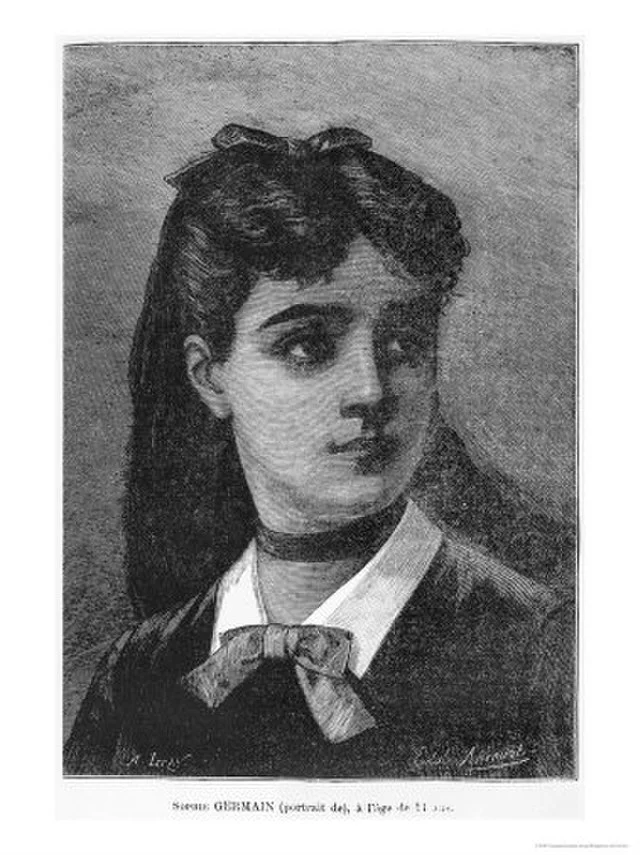
\includegraphics[width=.6\linewidth]{FIG/06-Sophie-Germain.png} 
\end{center}
}

\end{His}

\begin{ExoDec}{Compétence.}{1234}{1}{0}{0}{0}
% Un exercice de découverte/d'accroche
\end{ExoDec}
}

%%%%%%%%%%%%%%%%%%%%%%%%%%%%%%%%%%%%%%%%%%%%%%%%%%%%%%%%%%%%%%%%%%%
%%%% Page de cours 1
%%%%%%%%%%%%%%%%%%%%%%%%%%%%%%%%%%%%%%%%%%%%%%%%%%%%%%%%%%%%%%%%%%%

\begin{pageCours} % Début page de cours 1

\newgeometry{left=2cm,right=.8cm,top=1.5cm} %Ne pas toucher cette ligne

\section{Fonctions paires, fonctions impaires}

\mini{.5\linewidth}{
\begin{DefT}{Fonction paire}
On dit qu'une fonction $f$ est \textbf{paire} si :

\begin{itemize}
\item $\forall x\in D_f,-x\in D_f$
\item $\forall x\in D_f, f(-x)=f(x)$
\end{itemize}
\end{DefT}

\begin{Rq}
La \textbf{courbe représentative} d'une fonction pair est \textbf{symétrique} par rapport à l'\textbf{axe des ordonnées}.
\end{Rq}
}{.5\linewidth}{
\begin{center}
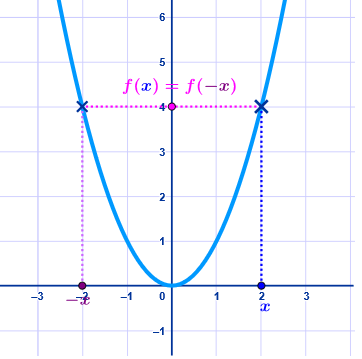
\includegraphics[width=.6\linewidth]{FIG/fonction_paire.png} 
\end{center}
}

\mini{.5\linewidth}{
\begin{DefT}{Fonction impaire}
On dit qu'une fonction $f$ est \textbf{impaire} si :

\begin{itemize}
\item $\forall x\in D_f,-x\in D_f$
\item $\forall x\in D_f, f(-x)=-f(x)$
\end{itemize}
\end{DefT}

\begin{Rq}
La \textbf{courbe représentative} d'une fonction pair est \textbf{symétrique} par rapport à l'\textbf{origine du repère}.
\end{Rq}
}{.5\linewidth}{
\begin{center}
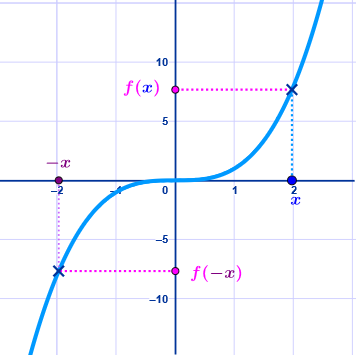
\includegraphics[width=.6\linewidth]{FIG/fonction_impaire.png} 
\end{center}
}

\section{La fonction Carré}

\begin{DefT}{Fonction Carré}\index{Fonctions!Carré}
La \textbf{fonction Carré} $f$ est la fonction définie sur $\mathbb{R}$ par $f(x)=x^2$.
 
La \textbf{représentation graphique} de la fonction Carré s'appelle une \textbf{parabole}\index{Parabole} et son équation est $y=x^2$. 
\end{DefT}

\begin{minipage}{0.48\linewidth}
\begin{Th} 
La fonction Carré $f$ est paire.

La parabole d'équation $y=x^2$ est symétrique par rapport à l'axe des ordonnées.
\end{Th}

\begin{ThT}{Variations de la fonction Carré}

\textcolor{red}{Démonstration exigible}

La fonction Carré est strictement décroissante sur $\mathbb{R}^-$ et strictement croissante sur $\mathbb{R}^+$. 

\begin{tikzpicture}
\tkzTabInit[lgt=1,espcl=2]{ $x$ / 1,$f $ / 2}
{ $-\infty$ , $0$ ,$+\infty$}
\tkzTabVar{+/$ $,-/$0$,+/$ $ }
\end{tikzpicture}

\end{ThT}

\end{minipage}
\hfill
\begin{minipage}{0.48\linewidth}

%\begin{Ill}
%\definecolor{xfqqff}{rgb}{0.4980392156862745,0.,1.}
%\begin{tikzpicture}[line cap=round,line join=round,>=triangle 45,x=0.7772020725388601cm,y=0.7772020725388601cm]
%\begin{axis}[
%x=0.7772020725388601cm,y=0.7772020725388601cm,
%axis lines=middle,
%ymajorgrids=true,
%xmajorgrids=true,
%xmin=-3.2800000000000002,
%xmax=3.42,
%ymin=-0.8400000000000007,
%ymax=7.079999999999996,
%xtick={-3.0,-2.0,...,3.0},
%ytick={0,1.0,...,7.0},]
%\clip(-3.28,-0.84) rectangle (3.42,7.08);
%\draw [color=xfqqff](1.3,1.84) node[anchor=north west] {$y=x^2$};
%\draw[line width=2.pt,color=xfqqff,smooth,samples=100,domain=-3.2800000000000002:3.42] plot(\x,{(\x)*(\x)});
%\begin{scriptsize}
%\draw[color=xfqqff] (-2.96,8.93) node {$g$};
%\end{scriptsize}
%\end{axis}
%\end{tikzpicture}
%%\end{Ill}
\begin{Pv}
Etude des variations de $f:x\mapsto x^2$ sur $[0;+\infty[$ :

Soient $a$ et $b$ deux nombres appartenant à $[0;+\infty[$ tels que $a<b$. 

Comparons les images de $a$ et $b$ par la fonction $f$.

$f(a)=a^2$ et $f(b)=b^2$

Pour les comparer on étudie le signe de leur différence :

$f(a)-f(b)=a^2-b^2=(a+b)(a-b)$

\begin{itemize}
\item $a$ et $b$ appartiennent à $[0;+\infty[$ donc $a+b>0$
\item $a<b$ donc $a-b<0$
\item $(a+b)(a-b)<0\Rightarrow a^2-b^2<0 \Rightarrow f(a)<f(b) \Rightarrow f(a)<f(b)$
\end{itemize}

Les images de $a$ et $b$ par la fonction $f$ sont rangés dans le même ordre que ces nombres. La fonction est donc croissante sur $[0;+\infty[$.

\end{Pv}
\end{minipage}

\end{pageCours} % Fin page de cours 1

\begin{pageAD}

\Sf{Parité d'une fonction}

\begin{ExoCad}{Représenter. Raisonner.}{1234}{0}{0}{0}{0}{0}

Déterminer si les fonctions suivantes sont paires ou impaires.

\begin{center}
\begin{tikzpicture}[line cap=round,line join=round,>=triangle 45,x=.7cm,y=.7cm]
\begin{axis}[
x=.7cm,y=.7cm,
axis lines=middle,
ymajorgrids=true,
xmajorgrids=true,
xmin=-5.987525829224177,
xmax=5.987964363878517,
ymin=-3.9956200100092336,
ymax=3.9880401187258965,
xtick={-5.0,-4.0,...,5.0},
ytick={-3.0,-2.0,...,3.0},]
\clip(-5.987525829224177,-3.9956200100092336) rectangle (5.987964363878517,3.9880401187258965);
\draw[line width=2.pt,color=sacado_orange,smooth,samples=100,domain=-5.987525829224177:5.987964363878517] plot(\x,{0-sin(((\x)/2)*180/pi)*3});
\end{axis}
\end{tikzpicture}
\begin{tikzpicture}[line cap=round,line join=round,>=triangle 45,x=.7cm,y=.7cm]
\begin{axis}[
x=.7cm,y=.7cm,
axis lines=middle,
ymajorgrids=true,
xmajorgrids=true,
xmin=-5.987525829224177,
xmax=5.987964363878517,
ymin=-3.9956200100092336,
ymax=3.9880401187258965,
xtick={-5.0,-4.0,...,5.0},
ytick={-3.0,-2.0,...,3.0},]
\clip(-5.987525829224177,-3.9956200100092336) rectangle (5.987964363878517,3.9880401187258965);
\draw[line width=2.pt,color=sacado_orange,smooth,samples=100,domain=-9.161981166126003:11.063291160002994] plot(\x,{sqrt((\x)^(2)+1)-2});
\end{axis}
\end{tikzpicture}
\end{center}\vspace{.2cm}

La fonction est .\dotfill La fonction est .\dotfill

\end{ExoCad} 

\begin{ExoCad}{Raisonner.}{1234}{0}{0}{0}{0}{0}
A partir de la définition, démontrer que la fonction $f:x\mapsto x^2$ est \textbf{paire}.

\point{3}

%La fonction $f$ est définie sur l'ensemble des réels, ainsi : $\forall x\in D_f,-x\in D_f$.
%
%Montrons que l'image de $-x$ par la fonction $f$ est égale à l'image de $x$.
%
%$f(-x)=(-x)^2=(-x)\times(-x)=x^2=f(x)$.
%
%Ainsi, la fonction $f :x\mapsto x^2$ est paire.
\end{ExoCad} 

\Sf{Connaitre et utiliser la fonction Carré}

\begin{ExoCad}{Raisonner.}{1234}{0}{0}{0}{0}{0}

Comparer sans les calculer.
\begin{description}[leftmargin=*]
\item $\left( \dfrac{3}{2} \right)^2$ et  $\pi^2$

%La fonction Carré est croissante sur $[0;+\infty]$, donc les images de deux nombres de $[0;+\infty]$ sont rangées dans le même ordre que ces nombres. Or comme $\dfrac{3}{2}<\pi$ alors $\dfrac{3}{2}^2<\pi^2$.

\point{2}

\item $(-11)^2$ et $(-6)^2$

%La fonction Carré est décroissante sur $[-\infty,0]$, donc les images de deux nombres de $[-\infty,0]$ sont rangées dans l'ordre contraire de ces nombres. Or comme $-11<-6$ alors $(-11)^2>(-6)^2$.

\point{2}

 
\item $-7^2$ et $-8^2$

%La fonction Carré est croissante sur $[0;+\infty]$, donc les images de deux nombres de $[0;+\infty]$ sont rangées dans le même ordre que ces nombres. Or comme $7<8$ alors $7^2<8^2$. Prendre l'opposé de deux nombres revient à prendre l'ordre contraire que ces nombres, ainsi : $-7^2>-8^2$.

\point{3}
\end{description}

\end{ExoCad} 


\begin{ExoCad}{Raisonner. Calculer.}{1234}{0}{0}{0}{0}{0}
\begin{itemize}[leftmargin=*]
\item Déterminer algébriquement l'intervalle de $x^2$ lorsque $x$ appartient à $[1;3]$. 

\point{2}

%La fonction $x\mapsto x^2$ est strictement croissante sur l'intervalle $[1;3]$. De plus $x$ est positif sur cet intervalle.
%
%$\textcolor{white}{\Leftrightarrow}1<x<3$
%
%$\Leftrightarrow1^2<x^2<3^2$
%
%$\Leftrightarrow1<x^2<9$
%
%Ainsi l'intervalle de $x^2$ lorsque $x$ appartient à $[1;3]$ est $[1;9]$.
\item Déterminer algébriquement l'intervalle de $x^2$ lorsque $x$ appartient à $\left[-1;4 \right]$. 

\point{3}

%La fonction $x\mapsto x^2$ est décroissante sur l'intervalle $[-1;0]$ puis croissante sur l'intervalle $[0;4]$. Traitons les deux intervalles séparément :
%
%\mini{.47\linewidth}{
%Sur $[-1;0]$, $x$ est négatif.
%
%$\textcolor{white}{\Leftrightarrow}-1<x<0$
%
%$\Leftrightarrow(-1)^2>x^2>0^2$
%
%$\Leftrightarrow1>x^2>0$
%
%Ainsi l'intervalle de $x^2$ lorsque $x$ appartient à $[-1;0]$ est $[0;1]$.
%}{.47\linewidth}{
%Sur $[0;4]$, $x$ est positif.
%
%$\textcolor{white}{\Leftrightarrow}0<x<4$
%
%$\Leftrightarrow0^2<x^2<4^2$
%
%$\Leftrightarrow0<x^2<16$
%
%Ainsi l'intervalle de $x^2$ lorsque $x$ appartient à $[0;4]$ est $[0;16]$.
%}
%
%Donc lorsque $x\in[-1,0]\cup[0,4]$, $x^2\in[0,1]\cup[0,16]$, cet intervalle peut se simplifier en $[0,16]$.

\end{itemize}

\end{ExoCad}

\end{pageAD}

\begin{pageCours} 

\section{La fonction Cube}

\begin{DefT}{Fonction Cube}\index{Inverse!Fonction}
La \textbf{fonction Cube} $f$ est la fonction définie sur $\mathbb{R}$ par $f(x)=x^3$.

\end{DefT}

\begin{minipage}{0.48\linewidth}
\begin{Th} 
La fonction Cube $f$ est impaire.

La courbe d'équation $y=x^3$ est symétrique par rapport à l'origine du repère.
\end{Th}


\begin{ThT}{Variations de la fonction Cube}

La fonction Cube est strictement  croissante sur $\mathbb{R}^-$ et strictement  croissante sur $\mathbb{R}^+$. 

\begin{tikzpicture}
\tkzTabInit[lgt=1,espcl=2]{ $x$ / 1,$f $ / 2}
{ $-\infty$ , $0$ ,$+\infty$}
\tkzTabVar{+/$ $,-/$0$,+/$ $ }
\end{tikzpicture}

\end{ThT}

\end{minipage}
\hfill
\begin{minipage}{0.48\linewidth}

%\begin{Ill}
\definecolor{xfqqff}{rgb}{0.4980392156862745,0.,1.}
\begin{tikzpicture}[line cap=round,line join=round,>=triangle 45,x=0.7772020725388601cm,y=0.7772020725388601cm]
\begin{axis}[
x=0.7772020725388601cm,y=0.7772020725388601cm,
axis lines=middle,
ymajorgrids=true,
xmajorgrids=true,
xmin=-3.4,
xmax=3.3200000000000003,
ymin=-5.199999999999999,
ymax=5.139999999999999,
xtick={-3.0,-2.0,...,3.0},
ytick={-5.0,-4.0,...,5.0},]
\clip(-3.4,-5.2) rectangle (3.32,5.14);
\draw [color=xfqqff](1.3,1.84) node[anchor=north west] {$y=x^3$};
\draw[line width=2.pt,color=xfqqff,smooth,samples=100,domain=-3.4:3.3200000000000003] plot(\x,{(\x)*(\x)*(\x)});
\end{axis}
\end{tikzpicture}
%%\end{Ill}

\end{minipage}

\section{{Positions relatives des courbes de $x$, $x^2$ et $x^3$}}

\mini{.7\linewidth}{
\begin{Pp}
\textcolor{red}{Démonstration exigible}

\begin{itemize}
\item Si $0\leq x \leq 1$ alors $x\geq x^2 \geq x^3$.
\item Si $x\geq 1$ alors $x\leq x^2 \leq x^3$
\end{itemize}

\begin{tikzpicture}
   \tkzTabInit{$x$ / 1 , $x$ / 1, $x-1$ / 1, $f(x)$ / 1}{$-\infty$, $0$, $1$, $+\infty$}
   \tkzTabLine{, -, z, +, t, +, }
   \tkzTabLine{, -, t, -, z, +, }
   \tkzTabLine{, +, z, -, z, +, }
\end{tikzpicture}
\end{Pp}

\begin{Pv}
Comparaison de $x$ et $x^2$ sur $[0;+\infty[$.

Pour les comparer, on étudie le signe de leur différence.

On définit la fonction $f$ par $f(x)=x^2-x$.

$f(x)=x^2-x=x(x-1)$

On peut établir le tableau de signes de $f(x)$.

$(E):f(x)=0$ alors $S(E)=\{0;1\}$\vspace{.2cm}

\begin{tikzpicture}
   \tkzTabInit{$x$ / 1 , $x$ / 1, $x-1$ / 1, $f(x)$ / 1}{$-\infty$, $0$, $1$, $+\infty$}
   \tkzTabLine{, -, z, +, t, +, }
   \tkzTabLine{, -, t, -, z, +, }
   \tkzTabLine{, +, z, -, z, +, }
\end{tikzpicture}

Ainsi :
\begin{itemize}
\item $\forall x \in ]0;1[,f(x)<0$ donc $x^2-x<0$ donc $x^2<x$
\item $\forall x \in ]1;+\infty,f(x)>0$ donc $x^2-x>0$ donc $x^2>x$
\end{itemize}
\end{Pv}
}{.3\linewidth}{
\begin{center}
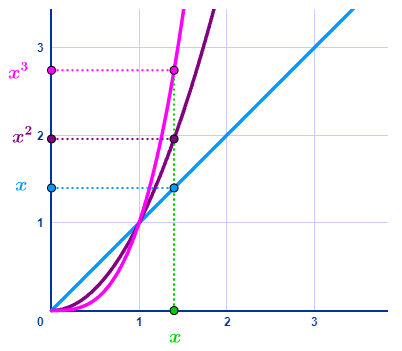
\includegraphics[width=\linewidth]{FIG/position_relative.png}
\end{center}
}



\end{pageCours} % Fin page de cours 2

%%%%%%%%%%%%%%%%%%%%%%%%%%%%%%%%%%%%%%%%%%%%%%%%%%%%%%%%%%%%%%%%%%%
%%%% Application direct 1
%%%%%%%%%%%%%%%%%%%%%%%%%%%%%%%%%%%%%%%%%%%%%%%%%%%%%%%%%%%%%%%%%%%

\begin{pageAD}  % Début page d'exercice d'application direct 1
\restoregeometry %Ne pas toucher cette ligne
 
\Sf{Connaitre et utiliser la fonction Cube}

\begin{ExoCad}{Raisonner.}{1234}{0}{0}{0}{0}{0}

A partir de la définition, démontrer que la fonction $f:x\mapsto x^3$ est \textbf{impaire}.

\point{3}

%La fonction $f$ est définie sur l'ensemble des réels, ainsi : $\forall x\in D_f,-x\in D_f$.
%
%Montrons que l'image de $-x$ par la fonction $f$ est égale à l'inverse de l'image de $x$.
%
%$f(-x)=(-x)^3=(-x)\times(-x)\times(-x)=x^2\times(-x)=-x^3=-f(x)$.
%
%Ainsi, la fonction $f :x\mapsto x^3$ est impaire.

\end{ExoCad} 

\begin{ExoCad}{Raisonner.}{1234}{0}{0}{0}{0}{0}

Comparer sans les calculer.

\begin{description}[leftmargin=*]
\item $\left(\frac{1}{5}\right)^3$ et $\pi^3$  

%La fonction cube est croissante sur $\mathbb{R}$, donc les cubes de deux nombres réels sont rangés dans le même ordre que ces nombres.
%
%On sait que $\dfrac{1}{5}=0,2$ et que $\pi\approx3$, or comme $\frac{1}{5}<\pi$ alors $\frac{1}{5}^3<\pi^3$

\point{2}

\item $(-5)^3$ et $(-9)^3$

%La fonction cube est croissante sur $\mathbb{R}$, donc les cubes de deux nombres réels sont rangés dans le même ordre que ces nombres.
%
%On sait que $-9>-5$ alors $(-9)^3<(-5)^3$.

\point{2}
\end{description}

\end{ExoCad} 

\Sf{Position relatives des courbes}

\begin{ExoCad}{Raisonner. Communiquer.}{1234}{0}{0}{0}{0}{0}

Comparer la position relative des courbes de $x^2$ et $x^3$ sur $[0;+\infty]$.

\point{5}

%Pour comparer la position relative des courbes de $x^2$ et $x^3$ on étudie le signe de leur différence.
%
%On définit la fonction $f$ par $f(x)=x^3-x^2=x^2(x-1)$
%
%On peut établir le tableau de signe de $f(x)$.
%
%$(E):f(x)=0$ alors $S(E)=\{0;1\}$
%
%\begin{tikzpicture}
%   \tkzTabInit{$x$ / 1 , $x^2$ / 1, $x-1$ / 1, $f(x)$ / 1}{$-\infty$, $0$, $1$, $+\infty$}
%   \tkzTabLine{, +, z, +, t, +, }
%   \tkzTabLine{, -, t, -, z, +, }
%   \tkzTabLine{, -, z, -, z, +, }
%\end{tikzpicture}
%
%Ainsi :
%
%\begin{itemize}
%\item $\forall x \in ]0;1[,f(x)<0$ donc $x^3-x^2<0$ donc $x^3<x^2$
%\item $\forall x \in ]1;+\infty,f(x)>0$ donc $x^3-x^2>0$ donc $x^3>x^2$
%\end{itemize}

\end{ExoCad} 

\begin{ExoCad}{Raisonner.}{1234}{0}{0}{0}{0}{0}

Comparer sans les calculer.

\begin{description}[leftmargin=*]
\item $(\frac{1}{3})^3$ et $(\frac{1}{3})^2$  



\point{2}

\item $\frac{10}{9}$ et $(\frac{10}{9})^2$



\point{2}
\end{description}

\end{ExoCad} 

 
\end{pageAD} % Fin page d'exercice d'application direct 1

%%%%%%%%%%%%%%%%%%%%%%%%%%%%%%%%%%%%%%%%%%%%%%%%%%%%%%%%%%%%%%%%%%%
%%%% Page de cours 2
%%%%%%%%%%%%%%%%%%%%%%%%%%%%%%%%%%%%%%%%%%%%%%%%%%%%%%%%%%%%%%%%%%%

\begin{pageCours} % Début page de cours 2

\newgeometry{left=2cm,right=.8cm,top=1.5cm} %Ne pas toucher cette ligne

\section{La fonction Inverse}



\begin{DefT}{Fonction Inverse}\index{Inverse!Fonction}
La \textbf{fonction Inverse} $f$ est la fonction définie sur $\mathbb{R}^*$ par $f(x)=\dfrac{1}{x}$.
 
La \textbf{représentation graphique} de la fonction Inverse s'appelle une \textbf{hyperbole}\index{hyperbole} et son équation est $y=\dfrac{1}{x}$. 
\end{DefT}

\begin{minipage}{0.48\linewidth}
\begin{Th} 
La fonction Inverse $f$ est impaire.

La hyperbole d'équation $y=\dfrac{1}{x}$ est symétrique par rapport à l'origine du repère.
\end{Th}


\begin{ThT}{Variations de la fonction Inverse}

\textcolor{red}{Démonstration exigible}

La fonction Carré est strictement décroissante sur $\mathbb{R}^*_-$ et strictement décroissante sur $\mathbb{R}^*_+$. 

\begin{tikzpicture}
\tkzTabInit[lgt=1,espcl=2]{ $x$ / 1,$f $ / 2}
{ $-\infty$ , $0$ ,$+\infty$}
\tkzTabVar{+/$0$ , -D+ /$ $/$ $ , -/$0$}
\end{tikzpicture}

\end{ThT}

\end{minipage}
\hfill
\begin{minipage}{0.48\linewidth}

%\begin{Ill}
\definecolor{xfqqff}{rgb}{0.4980392156862745,0.,1.}
\begin{tikzpicture}[line cap=round,line join=round,>=triangle 45,x=0.7772020725388601cm,y=0.7772020725388601cm]
\begin{axis}[
x=0.7772020725388601cm,y=0.7772020725388601cm,
axis lines=middle,
ymajorgrids=true,
xmajorgrids=true,
xmin=-4.5200000000000005,
xmax=5.6000000000000005,
ymin=-4.4799999999999995,
ymax=4.499999999999999,
xtick={-4.0,-3.0,...,5.0},
ytick={-4.0,-3.0,...,4.0},]
\clip(-4.52,-4.48) rectangle (5.6,4.5);
\draw [color=xfqqff](0.62,3.38) node[anchor=north west] {$y=\dfrac{1}{x}$};
\draw[line width=2.pt,color=xfqqff,smooth,samples=100,domain=-4.5200000000000005:-0.1] plot(\x,{1/(\x)});
\draw[line width=2.pt,color=xfqqff,smooth,samples=100,domain=0.1:5.6000000000000005] plot(\x,{1/(\x)});

\end{axis}
\end{tikzpicture}
%%\end{Ill}

\end{minipage}

\begin{Pv}
Étude des variations $f:x\mapsto \frac{1}{x}$ sur $]-\infty;0[$.

Soient $a$ et $b$ deux nombres appartenant à $]-\infty;0[$ tels que $a<b$.

Comparons les images de $a$ et $b$ par la fonction $f$.

$f(a)=\frac{1}{a}$ et $f(b)=\frac{1}{b}$

Pour les comparer on étudie le signe de leur différence.

$f(a)-f(b)=\frac{1}{a}-\frac{1}{b}=\frac{b}{ab}-\frac{a}{ab}=\frac{b-a}{ab}$

\begin{itemize}
\item $a$ et $b$ appartiennent à $]-\infty;0[$ donc $ab>0$
\item $a<b$ donc $a-b<0$ donc $b-a>0$
\item $\frac{b-a}{ab}>0\Rightarrow \frac{1}{a}-\frac{1}{b}>0 \Rightarrow f(a)-f(b)>0 \Rightarrow f(a)>f(b)$
\end{itemize}

Les images de $a$ et $b$ par la fonction $f$ sont rangés dans l'ordre contraire de celui de ces nombres. La fonction inverse est donc décroissante sur $]-\infty;0[$.
\end{Pv}

\section{La fonction Racine carrée}

\begin{DefT}{Fonction Racine carrée}\index{Racine carrée!Fonction}
La \textbf{fonction Racine carrée} $f$ est la fonction définie sur $\mathbb{R}^+$ par $f(x)=\sqrt{x}$.
\end{DefT}

\begin{Rq} 
L'ensemble de définition de la fonction Racine Carrée n'est pas centré. Donc la fonction Racine carrée n'est ni paire, ni impaire.
\end{Rq}

\begin{minipage}{0.48\linewidth}



\begin{ThT}{Variations de la fonction Racine Carrée}

\textcolor{red}{Démonstration exigible}

La fonction Racine carrée est strictement croissante sur $\mathbb{R}^+$. 

\begin{tikzpicture}
\tkzTabInit[lgt=1,espcl=2]{ $x$ / 1,$f $ / 2}
{ $-\infty$ , $0$ ,$+\infty$}
\tkzTabVar{+/$ $,-/$0$,+/$ $ }
\end{tikzpicture}

\end{ThT}

\end{minipage}
\hfill
\begin{minipage}{0.48\linewidth}

%\begin{Ill}
\definecolor{xfqqff}{rgb}{0.4980392156862745,0.,1.}
\begin{tikzpicture}[line cap=round,line join=round,>=triangle 45,x=0.7772020725388601cm,y=0.7772020725388601cm]
\begin{axis}[
x=0.7772020725388601cm,y=0.7772020725388601cm,
axis lines=middle,
ymajorgrids=true,
xmajorgrids=true,
xmin=-2.48,
xmax=7.24,
ymin=-0.78,
ymax=3.3000000000000003,
xtick={-2.0,-1.0,...,7.0},
ytick={-0.0,1.0,...,3.0},]
\clip(-2.48,-0.78) rectangle (7.24,3.3);
\draw [color=xfqqff](5.08,2.38) node[anchor=north west] {$y=\sqrt{x}$};
\draw[line width=2.pt,color=xfqqff,smooth,samples=100,domain=3.6799999990328158E-6:7.24] plot(\x,{sqrt((\x))});
\end{axis}
\end{tikzpicture}
%%\end{Ill}

\end{minipage}

\begin{Pv}
Etude des variations de $f:x\mapsto \sqrt{x}$ sur $[0;+\infty[$.

Soient $a$ et $b$ deux nombres appartenant à $[0;+\infty[$ tels que $a<b$.

Comparons les images de $a$ et $b$ par la fonction $f$.

$f(a)=\sqrt{a}$ et $f(b)=\sqrt{b}$

Pour les comparer on étudie le signe de leur différence.

$f(a)-f(b)=\sqrt{a}-\sqrt{b}=(\sqrt{a}-\sqrt{b})\times\frac{\sqrt{a}+\sqrt{b}}{\sqrt{a}+\sqrt{b}}=\frac{(\sqrt{a}-\sqrt{b})(\sqrt{a}+\sqrt{b})}{\sqrt{a}+\sqrt{b}}=\frac{\sqrt{a}^2-\sqrt{b}^2}{\sqrt{a}+\sqrt{b}}=\frac{a-b}{\sqrt{a}+\sqrt{b}}$

\begin{itemize}
\item $\sqrt{a}+\sqrt{b}>0$
\item $a<b$ donc $a-b<0$
\item $\frac{a-b}{\sqrt{a}+\sqrt{b}}<0\Rightarrow \sqrt{a}-\sqrt{b}<0 \Rightarrow f(a)-f(b)<0 \Rightarrow f(a)<f(b)$
\end{itemize}

Les images de $a$ et $b$ par la fonction $f$ sont rangés dans le même ordre que celui de ces nombres. La fonction racine carrée est donc croissante sur $[0;+\infty[$. 
\end{Pv}

\end{pageCours} % Fin page de cours 2

%%%%%%%%%%%%%%%%%%%%%%%%%%%%%%%%%%%%%%%%%%%%%%%%%%%%%%%%%%%%%%%%%%%
%%%% Application direct 2
%%%%%%%%%%%%%%%%%%%%%%%%%%%%%%%%%%%%%%%%%%%%%%%%%%%%%%%%%%%%%%%%%%%

\begin{pageAD}  % Début page d'exercice d'application direct 2
\restoregeometry %Ne pas toucher cette ligne

\Sf{Connaitre et utiliser les fonctions Inverse et Racine Carrée}

\begin{ExoCad}{Raisonner.}{1234}{0}{0}{0}{0}{0}

A partir de la définition, démontrer que la fonction $f:x\mapsto \frac{1}{x}$ est \textbf{impaire}.

\point{3}

%La fonction $f$ est définie sur l'ensemble des réels privé de $0$, ainsi : $\forall x\in D_f,-x\in D_f$.
%
%Montrons que l'image de $-x$ par la fonction $f$ est égale à l'inverse de l'image de $x$.
%
%$f(-x)=\frac{1}{-x}=-(\frac{1}{x})=-f(x)$.
%
%Ainsi, la fonction $f :x\mapsto \frac{1}{x}$ est impaire.

\end{ExoCad} 

\begin{ExoCad}{Raisonner.}{1234}{0}{0}{0}{0}{0}

Comparer sans les calculer.
\begin{description}[leftmargin=*]
\item $\dfrac{1}{5}$ et $\dfrac{1}{4}$  

\point{2}

%La fonction inverse est décroissante sur $]0;+\infty[$ donc les inverses de deux nombres strictement positifs sont rangés dans l'ordre contraire de ces nombres. Or comme $5>4$ alors $\dfrac{1}{5}<\dfrac{1}{4}$.

\item $-\dfrac{1}{4}$ et $-\dfrac{1}{6}$ 

\point{3}

%La fonction inverse est décroissante sur $]-\infty,0[$ donc les inverses de deux nombres strictement négatifs sont rangés dans l'ordre contraire de ces nombres. Or comme $-4<-6$ alors $-\dfrac{1}{4}>-\dfrac{1}{6}$.

\item $\sqrt{10}$ et $\sqrt{100}$ 

%La fonction racine carrée est croissante sur $]0;+\infty[$ donc la racine carrée de deux nombres sur cet intervalle sont rangés dans le même ordre que ces nombres. Or comme $10<100$ alors $\sqrt{10}<\sqrt{100}$.

\point{2}


\end{description}

\end{ExoCad} 


\begin{ExoCadN}{Raisonner.}{0}{0}{0}{0}{0}

Expliquer pourquoi la fonction Inverse n'est pas décroissante sur $\mathbb{R}^\ast$.

 \point{3}

%Si une fonction $f$ est décroissante sur un intervalle $I$, alors pour tous nombres de cet intervalle $a$ et $b$ tel que $a<b$ on a $f(a)>f(b)$. Prenons deux nombres sur $\mathbb{R}^\ast$ et vérifions la propriété : soit $-5$ et $3$ on a $-\dfrac{1}{5}<\dfrac{1}{3}$. Ces deux nombres ne vérifie pas la propriété donc la fonction inverse n'est pas décroissante sur $\mathbb{R}^\ast$.

\end{ExoCadN}
 

 

 

\begin{ExoCad}{Représenter. Raisonner.}{1234}{0}{0}{0}{0}{0}

Résoudre graphiquement les équations, puis retrouver les résultats algébriquement.
\begin{enumerate}[leftmargin=*]
\item $\frac{1}{x}=4$ 
\point{2}

%\definecolor{ffqqqq}{rgb}{1.,0.,0.}
%\definecolor{xfqqff}{rgb}{0.4980392156862745,0.,1.}
%\begin{tikzpicture}[line cap=round,line join=round,>=triangle 45,x=1.0cm,y=1.0cm]
%\begin{axis}[
%x=1.0cm,y=1.0cm,
%axis lines=middle,
%ymajorgrids=true,
%xmajorgrids=true,
%xmin=-2.985442306278779,
%xmax=3.873024152879434,
%ymin=-1.860081495738546,
%ymax=4.998384963419662,
%xtick={-2.0,-1.0,...,3.0},
%ytick={-1.0,0.0,...,4.0},]
%\clip(-2.985442306278779,-1.860081495738546) rectangle (3.873024152879434,4.998384963419662);
%\draw[line width=2.pt,color=xfqqff,smooth,samples=100,domain=-2.985442306278779:-0.01] plot(\x,{1/(\x)});
%\draw[line width=2.pt,color=xfqqff,smooth,samples=100,domain=0.01:3.873024152879434] plot(\x,{1/(\x)});
%\draw [line width=2.pt,color=ffqqqq,domain=-2.985442306278779:3.873024152879434] plot(\x,{(--4.-0.*\x)/1.});
%\begin{scriptsize}
%\draw[color=xfqqff] (-9.206361179092708,0.06222107520861367) node {$f$};
%\draw[color=ffqqqq] (-9.206361179092708,3.868186969445704) node {$g$};
%\draw [color=black] (0.25,4.)-- ++(-2.5pt,-2.5pt) -- ++(5.0pt,5.0pt) ++(-5.0pt,0) -- ++(5.0pt,-5.0pt);
%\draw[color=black] (1.2648749360164515,4.467095308132758) node {$A(0.25, 4)$};
%\end{scriptsize}
%\end{axis}
%\end{tikzpicture}
\item $\sqrt{x}=2$ 
\point{2}

%\begin{tikzpicture}[line cap=round,line join=round,>=triangle 45,x=1.0cm,y=1.0cm]
%\begin{axis}[
%x=1.0cm,y=1.0cm,
%axis lines=middle,
%ymajorgrids=true,
%xmajorgrids=true,
%xmin=-0.5824490948339428,
%xmax=9.386811339671995,
%ymin=-0.6405197872153475,
%ymax=3.4743091840740115,
%xtick={-0.0,1.0,...,9.0},
%ytick={-0.0,1.0,...,3.0},]
%\clip(-0.5824490948339428,-0.6405197872153475) rectangle (9.386811339671995,3.4743091840740115);
%\draw[line width=2.pt,color=xfqqff,smooth,samples=100,domain=4.946052066711085E-6:9.386811339671995] plot(\x,{sqrt((\x))});
%\draw [line width=2.pt,color=ffqqqq,domain=-0.5824490948339428:9.386811339671995] plot(\x,{(--2.-0.*\x)/1.});
%\begin{scriptsize}
%\draw[color=xfqqff] (0.03644794556323789,0.20419103819161438) node {$f$};
%\draw[color=ffqqqq] (-2.5060480041765314,1.8768857419677767) node {$g$};
%\draw [color=black] (4.,2.)-- ++(-2.5pt,-2.5pt) -- ++(5.0pt,5.0pt) ++(-5.0pt,0) -- ++(5.0pt,-5.0pt);
%\draw[color=black] (4.084369128701555,2.4790558353271948) node {$B(4, 2)$};
%\end{scriptsize}
%\end{axis}
%\end{tikzpicture}
\end{enumerate}
Valider ces résultats par le calcul.

\vspace{0.4cm}

\begin{minipage}{0.48\linewidth}
\point{3}
%Pour la première équation nous trouvons graphiquement : $x=0,25$, on vérifie que $\dfrac{1}{0,25}=4$.
\end{minipage}
\hfill
\begin{minipage}{0.48\linewidth}
\point{3}
%Pour la deuxième équation nous trouvons graphiquement : $x=4$, on vérifie que $\sqrt{4}=2$.
\end{minipage}

\end{ExoCad}


\begin{ExoCad}{Raisonner. Calculer.}{1234}{0}{0}{0}{0}{0}
\begin{enumerate}[leftmargin=*]
\item Déterminer algébriquement l'intervalle de $\dfrac{1}{x}$ lorsque $x$ appartient à $[1;3]$. 

\point{3}

%La fonction inverse est strictement monotone sur $[1;3]$, l'intervalle des images sera l'image de l'intervalle à savoir $[\dfrac{1}{3};\dfrac{1}{1}]$ autrement dit $[\dfrac{1}{3};1]$.

\item Déterminer algébriquement l'intervalle de $\sqrt{x}$ lorsque $x$ appartient à $\left[1;2 \right]$. 

\point{3}

%La fonction racine carrée est strictement monotone sur $[1,2]$, l'intervalle des images sera l'image de l'intervalle à savoir $[\sqrt{1};\sqrt{2}]$ autrement dit $[1;\sqrt{2}]$.
\end{enumerate}

\end{ExoCad}
 
\end{pageAD} % Fin page d'exercice d'application direct 2

%%%%%%%%%%%%%%%%%%%%%%%%%%%%%%%%%%%%%%%%%%%%%%%%%%%%%%%%%%%%%%%%%%%
%%%% Parcours niveau 1
%%%%%%%%%%%%%%%%%%%%%%%%%%%%%%%%%%%%%%%%%%%%%%%%%%%%%%%%%%%%%%%%%%%

\begin{pageParcoursu} % Début du parcours niveau 1

%Premier exo du parcours 1
\begin{ExoCuN}{Représenter. Raisonner.}{0}{0}{0}{0}{0}
Associer à chaque représentation la fonction de référence qui lui correspond.\vspace{.2cm}

\begin{center}
\begin{tikzpicture}[line cap=round,line join=round,>=triangle 45,x=.4cm,y=.4cm]
\begin{axis}[
x=.4cm,y=.4cm,
axis lines=middle,
ymajorgrids=true,
xmajorgrids=true,
xmin=-5,
xmax=5,
ymin=-5,
ymax=5,
xtick={-4.0,-2.0,...,4.0},
ytick={-4.0,-2.0,...,4.0},]
\clip(-5,-5) rectangle (5,5);
%\draw[line width=2.pt,smooth,samples=100,domain=-5:5] plot(\x,{(\x)^(2)});
\draw[line width=2.pt,smooth,samples=100,domain=-5:5] plot(\x,{(\x)^(3)});
%\draw[line width=2.pt,smooth,samples=100,domain=-5:5] plot(\x,{1/(\x)});
%\draw[line width=2.pt,smooth,samples=100,domain=.1:5] plot(\x,{sqrt((\x))});
\end{axis}
\end{tikzpicture}\hspace{.2cm}
\begin{tikzpicture}[line cap=round,line join=round,>=triangle 45,x=.4cm,y=.4cm]
\begin{axis}[
x=.4cm,y=.4cm,
axis lines=middle,
ymajorgrids=true,
xmajorgrids=true,
xmin=-5,
xmax=5,
ymin=-5,
ymax=5,
xtick={-4.0,-2.0,...,4.0},
ytick={-4.0,-2.0,...,4.0},]
\clip(-5,-5) rectangle (5,5);
%\draw[line width=2.pt,smooth,samples=100,domain=-5:5] plot(\x,{(\x)^(2)});
%\draw[line width=2.pt,smooth,samples=100,domain=-5:5] plot(\x,{(\x)^(3)});
%\draw[line width=2.pt,smooth,samples=100,domain=-5:5] plot(\x,{1/(\x)});
\draw[line width=2.pt,smooth,samples=100,domain=.01:5] plot(\x,{sqrt((\x))});
\end{axis}
\end{tikzpicture}\hspace{.2cm}
\begin{tikzpicture}[line cap=round,line join=round,>=triangle 45,x=.4cm,y=.4cm]
\begin{axis}[
x=.4cm,y=.4cm,
axis lines=middle,
ymajorgrids=true,
xmajorgrids=true,
xmin=-5,
xmax=5,
ymin=-5,
ymax=5,
xtick={-4.0,-2.0,...,4.0},
ytick={-4.0,-2.0,...,4.0},]
\clip(-5,-5) rectangle (5,5);
\draw[line width=2.pt,smooth,samples=100,domain=-5:5] plot(\x,{(\x)^(2)});
%\draw[line width=2.pt,smooth,samples=100,domain=-5:5] plot(\x,{(\x)^(3)});
%\draw[line width=2.pt,smooth,samples=100,domain=-5:5] plot(\x,{1/(\x)});
%\draw[line width=2.pt,smooth,samples=100,domain=.001:5] plot(\x,{sqrt((\x))});
\end{axis}
\end{tikzpicture}\hspace{.2cm}
\begin{tikzpicture}[line cap=round,line join=round,>=triangle 45,x=.4cm,y=.4cm]
\begin{axis}[
x=.4cm,y=.4cm,
axis lines=middle,
ymajorgrids=true,
xmajorgrids=true,
xmin=-5,
xmax=5,
ymin=-5,
ymax=5,
xtick={-4.0,-2.0,...,4.0},
ytick={-4.0,-2.0,...,4.0},]
\clip(-5,-5) rectangle (5,5);
%\draw[line width=2.pt,smooth,samples=100,domain=-5:5] plot(\x,{(\x)^(2)});
%\draw[line width=2.pt,smooth,samples=100,domain=-5:5] plot(\x,{(\x)^(3)});
\draw[line width=2.pt,smooth,samples=100,domain=-5:-0.01] plot(\x,{1/(\x)});
\draw[line width=2.pt,smooth,samples=100,domain=0.01:5] plot(\x,{1/(\x)});
%\draw[line width=2.pt,smooth,samples=100,domain=.1:5] plot(\x,{sqrt((\x))});
\end{axis}
\end{tikzpicture}
\end{center}\vspace{.2cm}

.\dotfill
\end{ExoCuN}

%Deuxième exo du parcours 1
\begin{ExoCuN}{Raisonner. Calculer.}{0}{0}{0}{0}{0}
Résoudre dans $\mathbb{R}$ les équations et inéquations suivantes :

\begin{enumerate}
\item $x^2=6$
\item $x^2=\frac{5}{3}$
\item $x^2\leq 3$
\item $\frac{1}{x}\geq1$
\end{enumerate}
\end{ExoCuN}

%Troisième exo du parcours 1
\begin{ExoCuN}{Compétence.}{1}{0}{0}{0}{0}
Associer à chaque courbe la fonction qui correspond :
\[f:x\mapsto 2x^2 \quad g:x\mapsto x^2+2 \quad h:x\mapsto x^2-1\]
\begin{center}
\begin{tikzpicture}[line cap=round,line join=round,>=triangle 45,x=.8cm,y=.8cm]
	\begin{axis}[
	x=.8cm,y=.8cm,
	axis lines=middle,
	ymajorgrids=true,
	xmajorgrids=true,
	xmin=-2.9997324598484885,
	xmax=3.0081249478055305,
	ymin=-1.9900228646581366,
	ymax=3.993754954187645,
	xtick={-2.0,-1.0,...,3.0},
	ytick={-1.0,0.0,...,3.0},]
\clip(-3,-2) rectangle (3.0081249478055305,3.993754954187645);
\draw[line width=2.pt,color=sacado_violet,smooth,samples=100,domain=-2.9997324598484885:3.0081249478055305] plot(\x,{(\x)^(2.0)+2});
\draw[line width=2.pt,color=sacado_blue,smooth,samples=100,domain=-2.9997324598484885:3.0081249478055305] plot(\x,{(\x)^(2)-1});
\draw[line width=2.pt,color=sacado_green,smooth,samples=100,domain=-2.9997324598484885:3.0081249478055305] plot(\x,{2*(\x)^(2)});
	\end{axis}
\end{tikzpicture}
\end{center}

\end{ExoCuN}

%Quatrième exo du parcours 1
\begin{ExoCuN}{Raisonner.}{1}{0}{0}{0}{0}
Dire si les phrases suivantes sont vraies ou fausses :
\begin{enumerate}
\item Un nombre et son carré ont toujours le même signe.
\item L'équation $x^2=k$ a toujours une solution.
\item La fonction $x\mapsto x^2$ sera toujours supérieure à $x\mapsto -1$.
\item Si $x\in[0,1]$ alors $x^2\in[0,1]$.
\end{enumerate}
\end{ExoCuN}

%Cinquième exo du parcours 1
\begin{ExoCuN}{Compétence.}{1}{0}{0}{0}{0}

\end{ExoCuN}

%Sixième exo du parcours 1
\begin{ExoCuN}{Compétence.}{1}{0}{0}{0}{0}

\end{ExoCuN}


\end{pageParcoursu} % Fin du parcours niveau 1
 
%%%%%%%%%%%%%%%%%%%%%%%%%%%%%%%%%%%%%%%%%%%%%%%%%%%%%%%%%%%%%%%%%%%
%%%% Parcours Niveau 2
%%%%%%%%%%%%%%%%%%%%%%%%%%%%%%%%%%%%%%%%%%%%%%%%%%%%%%%%%%%%%%%%%%%

\begin{pageParcoursd} % Début du parcours niveau 2

%Premier exo du parcours 2
\begin{ExoCdN}{Raisonner. Communiquer.}{0}{0}{0}{0}{0}

Démontrer que $f:x\mapsto x^2$ est décroissante sur $[-\infty;0[$.\vspace{.2cm}

\point{5}

\end{ExoCdN}

%Deuxième exo du parcours 2
\begin{ExoCdN}{Raisonner. Communiquer.}{0}{0}{0}{0}{0}
En utilisant la propriété de parité de la fonction $x\mapsto x^2$, montrer que $2x^2+3$ est paire.\vspace{.2cm}

\point{3}
\end{ExoCdN}

%Troisième exo du parcours 2
\begin{ExoCdN}{Raisonner. Calculer.}{2}{0}{0}{0}{0}
Résoudre dans $\mathbb{R}$ les équations et inéquations suivantes :

\begin{enumerate}
\item $x^2+3=4$
\item $\sqrt{x}=25$
\item $x^2\geq \frac{16}{36}$
\item $\frac{1}{x}\leq1$
\end{enumerate}
\end{ExoCdN}

%Quatrième exo du parcours 2
\begin{ExoCdN}{Raisonner.}{1}{0}{0}{0}{0}
Les hyperboles suivantes correspondent toutes à une fonction ayant la forme $x\mapsto \frac{k}{x}$. Analyser les courbes et identifier les fonctions :

\[f(x)=\frac{\ldots}{x}\hspace{1cm}g(x)=\frac{\ldots}{x}\hspace{1cm}h(x)=\frac{\ldots}{x}\]

\begin{center}
\definecolor{ffxfqq}{rgb}{1.,0.4980392156862745,0.}
\definecolor{ffvvqq}{rgb}{1.,0.3333333333333333,0.}
\definecolor{qqqqff}{rgb}{0.,0.,1.}
\definecolor{xfqqff}{rgb}{0.4980392156862745,0.,1.}
\begin{tikzpicture}[line cap=round,line join=round,>=triangle 45,x=1.0cm,y=1.0cm]
\begin{axis}[
x=1.0cm,y=1.0cm,
axis lines=middle,
ymajorgrids=true,
xmajorgrids=true,
xmin=-6.9930343163225785,
xmax=6.992498216875903,
ymin=-4.007317166218129,
ymax=4.00485492441223,
xtick={-6.0,-5.0,...,6.0},
ytick={-4.0,-3.0,...,4.0},]
\clip(-6.9930343163225785,-4.007317166218129) rectangle (6.992498216875903,4.00485492441223);
\draw[line width=2.pt,color=xfqqff,smooth,samples=100,domain=-6.9930343163225785:6.992498216875903] plot(\x,{5/(\x)});
\draw[line width=2.pt,color=qqqqff,smooth,samples=100,domain=-6.9930343163225785:6.992498216875903] plot(\x,{4/(\x)});
\draw[line width=2.pt,color=ffvvqq,smooth,samples=100,domain=-6.9930343163225785:6.992498216875903] plot(\x,{0-1/(\x)});
\draw [color=xfqqff](2.4141141650871423,2.8423745987627362) node[anchor=north west] {$\mathcal{C}_f$};
\draw [color=qqqqff](1.6093200934836491,2.0018119017546403) node[anchor=north west] {$\mathcal{C}_g$};
\draw [color=ffxfqq](-1.860236570762522,1.5368197714948428) node[anchor=north west] {$\mathcal{C}_h$};
\end{axis}
\end{tikzpicture}
\end{center}
\end{ExoCdN}

%Cinquième exo du parcours 2
\begin{ExoCdN}{Raisonner.}{0}{0}{0}{0}{0}
Dire si les phrases suivantes sont vraies ou fausses :
\begin{enumerate}
\item Un nombre et son cube ont toujours le même signe.
\item L'équation $\sqrt{x}=k$ admet toujours une solution.
\item La fonction $x\mapsto x^2$ n'admet pas de maximum.
\item La fonction inverse est décroissante sur $[-1,1]$.
\end{enumerate}
\end{ExoCdN}

%Sixième exo du parcours 2
\begin{ExoCdN}{Compétence.}{2}{0}{0}{0}{0}

\end{ExoCdN}

\end{pageParcoursd} % Fin du parcours niveau 2

%%%%%%%%%%%%%%%%%%%%%%%%%%%%%%%%%%%%%%%%%%%%%%%%%%%%%%%%%%%%%%%%%%%%
%%%%% Parcours Niveau 3
%%%%%%%%%%%%%%%%%%%%%%%%%%%%%%%%%%%%%%%%%%%%%%%%%%%%%%%%%%%%%%%%%%%%

\begin{pageParcourst} % Début du parcours niveau 3

% Cinquième exo du parcours 3
\begin{ExoCtN}{Raisonner.}{1}{1}{0}{0}{0}
Déterminer la parité de la fonction $f:x\mapsto \frac{1}{x^2+1}$.

\point{4}
\end{ExoCtN}

% Premier exo du parcours 3
\begin{ExoCtN}{Raisonner. Calculer}{1}{0}{0}{0}{0}
 Résoudre dans $\mathbb{R}$ les équations et inéquations suivantes :

\begin{enumerate}
\item $4x^2+3=8$
\item $2\sqrt{x}=72$
\item $x^2+2\leq 6$
\item $\frac{1}{x}-1\leq-2$
\end{enumerate}
\end{ExoCtN}

% Deuxième exo du parcours 3
\begin{ExoCtN}{Raisonner. Communiquer.}{1}{1}{0}{0}{0}
Sachant que $a^3-a^3=(a-b)(a^2+ab+b^2)$, montrer que $f:x\mapsto x^3$ est croissante sur $[0;+\infty[$.\vspace{.2cm}

\point{5}
 
\end{ExoCtN}

% Troisième exo du parcours 3
\begin{ExoCtN}{Raisonner.}{1}{1}{0}{0}{0}
Les courbes suivantes correspondent toutes à une fonction cubique, retrouver leur expressions.

\[f(x)=\ldots\ldots\ldots\hspace{1cm}g(x)=\ldots\ldots\ldots\hspace{1cm}h(x)=\ldots\ldots\ldots\]

 \definecolor{xfqqff}{rgb}{0.4980392156862745,0.,1.}
\definecolor{zzttqq}{rgb}{0.6,0.2,0.}
\definecolor{dcrutc}{rgb}{0.8627450980392157,0.0784313725490196,0.23529411764705882}
\definecolor{zzttff}{rgb}{0.6,0.2,1.}
\begin{tikzpicture}[line cap=round,line join=round,>=triangle 45,x=1.0cm,y=1.0cm]
\begin{axis}[
x=1.0cm,y=1.0cm,
axis lines=middle,
ymajorgrids=true,
xmajorgrids=true,
xmin=-2.9733677267582084,
xmax=2.9846155317648115,
ymin=-5.012969380833157,
ymax=5.018523198213632,
xtick={-2.0,-1.0,...,2.0},
ytick={-5.0,-4.0,...,5.0},]
\clip(-2.9733677267582084,-5.012969380833157) rectangle (2.9846155317648115,5.018523198213632);
\draw[line width=2.pt,color=zzttff,smooth,samples=100,domain=-2.9733677267582084:2.9846155317648115] plot(\x,{(\x)^(3)/2});
\draw[line width=2.pt,color=dcrutc,smooth,samples=100,domain=-2.9733677267582084:2.9846155317648115] plot(\x,{(\x)^(3)+1});
\draw[line width=2.pt,color=zzttqq,smooth,samples=100,domain=-2.9733677267582084:2.9846155317648115] plot(\x,{(\x)^(3)-2});
\draw [color=xfqqff](2.280317191300429,3.533786156153576) node[anchor=north west] {$\mathcal{C}_f$};
\draw [color=zzttqq](1.271457406310908,-0.5777933449358101) node[anchor=north west] {$\mathcal{C}_g$};
\draw [color=dcrutc](0.376808163018314,3.2672948921940788) node[anchor=north west] {$\mathcal{C}_h$};
\begin{scriptsize}
\draw[color=zzttff] (-2.17389393487972,-5.384153641348171) node {$f$};
\draw[color=dcrutc] (-1.8122272195061182,-5.36511855106535) node {$g$};
\draw[color=zzttqq] (-1.4695955944153376,-5.384153641348171) node {$h$};
\end{scriptsize}
\end{axis}
\end{tikzpicture}
\end{ExoCtN}

% Quatrième exo du parcours 3
\begin{ExoCtN}{Compétence.}{1}{1}{0}{0}{0}
 Dire si les phrases suivantes sont vraies ou fausses :
\begin{enumerate}
\item A partir de $x=1$ la courbe de $x^2$ est toujours comprise entre celles de $x^3$ et $x$.
\item 
\end{enumerate}
\end{ExoCtN}

% Cinquième exo du parcours 3
\begin{ExoCtN}{Compétence.}{1}{1}{0}{0}{0}
 
\end{ExoCtN}

% Sixième exo du parcours 3
\begin{ExoCtN}{Compétence.}{1}{1}{0}{0}{0}
 
\end{ExoCtN}
 
\end{pageParcourst} % Fin du parcours niveau 3

%%%%%%%%%%%%%%%%%%%%%%%%%%%%%%%%%%%%%%%%%%%%%%%%%%%%%%%%%%%%%%%%%%%
%%%%  Autoevaluation/exos ouverts
%%%%%%%%%%%%%%%%%%%%%%%%%%%%%%%%%%%%%%%%%%%%%%%%%%%%%%%%%%%%%%%%%%%

\begin{pageAuto} % Début de la page d'exos ouverts

%QCM
\begin{ExoAutoN}{Compétence.}{1}{0}{0}{0}{0}
\begin{tabular}{|c|c|c|c|}
\hline
Enoncé & A & B & C \\\hline
$f:\mapsto \frac{1}{x}$, sachant que $f(a)=-7,54$ que vaut $f(-a)$ ? & $f(-a)=-7,54$ & $f(-a)=7,54$ & On ne peut pas savoir \\\hline
\end{tabular}
\end{ExoAutoN}

\end{pageAuto} % Fin de la page d'exos ouverts

%%%%%%%%%%%%%%%%%%%%%%%%%%%%%%%%%%%%%%%%%%%%%%%%%%%%%%%%%%%%%%%%%%%
%%% Page algorithmique
%%%%%%%%%%%%%%%%%%%%%%%%%%%%%%%%%%%%%%%%%%%%%%%%%%%%%%%%%%%%%%%%%%%

\begin{pageAlgo} % Début de la page d'exos d'algorithmique

%Exercice d'algorithmique
\begin{ExoAlgoN}{Compétence.}{1}{0}{0}{0}{0}

\end{ExoAlgoN}

%Exercice d'algorithmique
\begin{ExoAlgo}{Compétence.}{1}{0}{0}{0}{0}

\end{ExoAlgo}

\end{pageAlgo} % Fin de la page d'exos d'algorithmique

%%%%%%%%%%%%%%%%%%%%%%%%%%%%%%%%%%%%%%%%%%%%%%%%%%%%%%%%%%%%%%%%%%%
%%%%  Page(s) blanche(s)
%%%%%%%%%%%%%%%%%%%%%%%%%%%%%%%%%%%%%%%%%%%%%%%%%%%%%%%%%%%%%%%%%%%

\begin{pageBrouillon}

\end{pageBrouillon}

\end{document}
